\documentclass[conference, compsoc]{IEEEtran}

\newif\ifExtended
\Extendedfalse

\usepackage{booktabs} % For formal tables
\usepackage{tikz}
\usetikzlibrary{shadows}
\usepackage{pgfplots}
\pgfplotsset{compat=1.10}

\usepackage{colortbl}
\definecolor{Gray}{gray}{0.925}

\usepackage{algorithm}
\usepackage{algorithmicx}
\usepackage{algpseudocode}
\usepackage[inline]{enumitem}
\usepackage{comment}
\usepackage{soul}
\usepackage{xspace}

\usepackage{amssymb}
\usepackage{amsmath}

\newcommand{\vect}[1]{\ensuremath{\boldsymbol{#1}}}
\newcommand{\va}{\vect{a}}
\newcommand{\vo}{\vect{o}}

\newcommand{\calA}[0]{\ensuremath{\mathcal{A}}}
\newcommand{\calC}[0]{\ensuremath{\mathcal{C}}}
\newcommand{\calO}[0]{\ensuremath{\mathcal{O}}}
\newcommand{\calP}[0]{\ensuremath{\mathcal{P}}}
\newcommand{\calR}[0]{\ensuremath{\mathcal{R}}}

\newcommand{\Natural}[0]{\ensuremath{\mathbb{N}}}
\newcommand{\Real}[0]{\ensuremath{\mathbb{R}}}

\usepackage{amsthm}

\theoremstyle{definition}
\newtheorem{definition}{Definition}


%-----Solidity Environment--------------------------------
\usepackage{listings, xcolor}
\definecolor{verylightgray}{rgb}{.97,.97,.97}
\lstdefinelanguage{Solidity}{
	keywords=[1]{anonymous, assembly, assert, balance, break, call, callcode, case, catch, class, constant, continue, contract, debugger, default, delegatecall, delete, do, else, event, export, external, false, finally, for, function, gas, if, implements, import, in, indexed, instanceof, interface, internal, is, length, library, log0, log1, log2, log3, log4, memory, modifier, new, payable, pragma, private, protected, public, pure, push, require, return, returns, revert, selfdestruct, send, storage, struct, suicide, super, switch, then, this, throw, transfer, true, try, typeof, using, value, view, while, with, addmod, ecrecover, keccak256, mulmod, ripemd160, sha256, sha3}, % generic keywords including crypto operations
	keywordstyle=[1]\color{blue}\bfseries,
	keywords=[2]{address,..., bool, byte, bytes, bytes1, bytes2, bytes3, bytes4, bytes5, bytes6, bytes7, bytes8, bytes9, bytes10, bytes11, bytes12, bytes13, bytes14, bytes15, bytes16, bytes17, bytes18, bytes19, bytes20, bytes21, bytes22, bytes23, bytes24, bytes25, bytes26, bytes27, bytes28, bytes29, bytes30, bytes31, bytes32, enum, int, int8, int16, int24, int32, int40, int48, int56, int64, int72, int80, int88, int96, int104, int112, int120, int128, int136, int144, int152, int160, int168, int176, int184, int192, int200, int208, int216, int224, int232, int240, int248, int256, mapping, string, uint, uint8, uint16, uint24, uint32, uint40, uint48, uint56, uint64, uint72, uint80, uint88, uint96, uint104, uint112, uint120, uint128, uint136, uint144, uint152, uint160, uint168, uint176, uint184, uint192, uint200, uint208, uint216, uint224, uint232, uint240, uint248, uint256, var, void, ether, finney, szabo, wei, days, hours, minutes, seconds, weeks, years},	% types; money and time units
	keywordstyle=[2]\color{teal}\bfseries,
	keywords=[3]{block, blockhash, coinbase, difficulty, gaslimit, number, timestamp, msg, data, gas, sender, sig, value, now, tx, gasprice, origin},	% environment variables
	keywordstyle=[3]\color{violet}\bfseries,
	identifierstyle=\color{black},
	sensitive=false,
	comment=[l]{//},
	morecomment=[s]{/*}{*/},
	commentstyle=\color{gray}\ttfamily,
	stringstyle=\color{red}\ttfamily,
	morestring=[b]',
	morestring=[b]"
}
\lstset{
	language=Solidity,
	backgroundcolor=\color{verylightgray},
	extendedchars=true,
	basicstyle=\footnotesize\ttfamily,
	showstringspaces=false,
	showspaces=false,
	numbers=left,
	numberstyle=\footnotesize,
	numbersep=1pt,
	tabsize=2,
	breaklines=true,
	showtabs=false,
	captionpos=b,
	xleftmargin=.5em,
	xrightmargin=.5em
}

\newcommand{\change}[2]{\st{#1} {\textcolor{blue}{#2}}}
\usepackage{caption}
\usepackage{subcaption}
\usepackage[textsize=tiny, textwidth=1.5cm,disable]{todonotes}
\newcommand{\TODO}[1]{\todo[inline]{#1}}
\newcommand{\ad}[1]{\todo[color=yellow!50, linecolor=black!50]{\textbf{Abhishek}: #1}}
\newcommand{\Aron}[1]{\todo[color=blue!25, linecolor=black!50]{\textbf{Aron}: #1}}
\newcommand{\Anastasia}[1]{\todo[color=pink, linecolor=black!50]{\textbf{Anastasia}: #1}}
\newcommand{\Scott}[1]{\todo[color=orange!30, linecolor=black!50]{\textbf{Scott}: #1}}

%\usepackage{hyperref}

\usepackage{url}
\graphicspath{{./figs/}}

\usepackage{titlesec}

\titlespacing\section{0pt}{8pt plus 4pt minus 2pt}{4pt plus 2pt minus 2pt}
\titlespacing\subsection{0pt}{8pt plus 4pt minus 2pt}{4pt plus 2pt minus 2pt}
\titlespacing\subsubsection{0pt}{8pt plus 4pt minus 2pt}{4pt plus 2pt minus 2pt}


\newcommand{\Platform}{\textit{SolidWorx}\xspace}

\begin{document}

\setlength{\marginparwidth}{1.4cm}

\thispagestyle{plain}
\pagestyle{plain}

\title{\Platform: A Resilient and Trustworthy Transactive Platform for\\Smart and Connected Communities}
\author{
\IEEEauthorblockN{Scott Eisele}
\IEEEauthorblockA{Vanderbilt University \\
Nashville, TN, USA \\ 
scott.r.eisele@vanderbilt.edu
}

\and
\IEEEauthorblockN{Aron Laszka}
\IEEEauthorblockA{University of Houston\\
Houston, TX, USA \\
alaszka@houston.edu}
\and
\IEEEauthorblockN{Anastasia Mavridou}
\IEEEauthorblockA{Vanderbilt University\\
Nashville, TN, USA \\
anastasia.mavridou@vanderbilt.edu}
\and
\IEEEauthorblockN{Abhishek Dubey}
\IEEEauthorblockA{Vanderbilt University \\
Nashville, TN, USA \\ 
abhishek.dubey@vanderbilt.edu
}
}

\maketitle

\begin{abstract}
Internet of Things and data sciences are fueling the development of innovative solutions for various applications in Smart and Connected Communities. These applications provide participants with the capability to exchange not only data but also resources, which raises the concerns of integrity, trust, and above all the need for fair and optimal solutions to the problem of resource allocation. Blockchain-based computational platforms may act as an enabling technology for these applications by providing immutability and distributed event chronology, enabling the implementation of ``higher-level contracts,'' which monitor system execution and provide guarantees on services that the rest of the system can depend upon. In this paper, we introduce the \Platform platform, which provides (a) distributed coordination and (b) decentralized market mechanisms as service. %We also describe the requirements and 
Based on case studies of energy trading and carpooling applications, we demonstrate the capabilities of \Platform.


% \textcolor{red}{the abstract has to be re-written}
% If the last decade viewed computational services as a \textit{utility}, 
% then surely this decade has transformed computation into a \textit{commodity}. Computation is now progressively integrated into physical networks in a seamless way, which enables smart and connected community applications to meet their latency requirements.  In this new  scenario, the boundaries between the network node, the sensor, and the actuator are blurring. Any node can be seen as part of a graph, with the capacity to serve as a computing or network router node (or both), and complex applications can possibly be distributed over this graph/network of nodes, so that the overall performance (e.g., amount of data processed over time) is significantly improved. However, the shared nature of resources and  the dependence on data-driven mechanisms make smart and connected community applications vulnerable. Classical, redundancy based mechanisms, such as self-checking pair and recovery blocks, are not applicable because of the dynamism and uncertainties---both endogenous (computation resources) and exogenous (environment). Blockchain based computational platforms may act as an enabling technology for these applications by providing immutability and distributed event chronology, enabling ``higher-level contracts'' to be written, which monitor system execution and provide guarantees on services that the rest of the system can depend upon. In this paper, we describe \Platform, which provides (a) distributed co-ordination and (b) decentralized market mechanisms as service. %We also describe the requirements and 
% Using case studies of energy distributed systems and carpooling, we demonstrate the capabilities of \Platform.
% %A use case of energy distribution systems is used as a casestudy. \Abhishek{title will be updated later.}
\end{abstract}
\setlength{\belowcaptionskip}{-10pt}
\section{Introduction}
\label{sec:intro}


%
% - motivation: in a smart and connected community, a number of stakeholders must collaborate and share/trade resources
%   * trust problem: stakeholders may have limited trust in each other
%   * distributed system problem: large number of stakeholder must cooperate and reach consensus on the state of the market
%   * auditability requirement: market must be transparent
%   * resilience problem: malicious or negligent stakeholder threaten the entire community 

% decentralized ledger and computational platform
% - challenges:
%   * efficiency <- large number of transaction must be cleared in short amount of time
%   * privacy <- personal information from residents
%   * correctness <- critical infrastructure for smart communities
%
Smart and connected communities (SCC) as a research area lies at the intersection of social science, machine learning, cyber-physical systems, civil infrastructures, and data sciences. This research area is  enabled by the rapid and transformational changes driven by  innovations in smart sensors, such as cameras and air quality monitors, which are now  embedded in almost every physical device and system that we use, ranging from watches and smartphones to automobiles, homes, roads, and workplaces. 
%Coupled with emerging new modes of networking, new algorithms for data analytics, and new paradigms of distributed computing like fog computing, these sensors create an ``Internet of Things'' (IoT)  that provide endless opportunities for innovation and improving the quality of life, such as improved transportation with reduced congestion and more efficient uses of energy and water. 
The effects of these innovations can be seen in a number of diverse domains, including transportation, energy, emergency response, and  health care, to name a few.


\ifExtended
At its core, smart and connected community applications are distributed programs where the results received by the end users or the performance that they experience is affected by others using the same application. A classical example of this kind is traffic routing,  implemented by many commercial mobility planning solutions, such as Waze and Google. The routes provided to the end users depend upon the interaction that other users in the systems have had with the application. An effective route planning solution will be proactive in the sense that it will analyze the demands being made by users and will use the dynamic demand model for effectively distributing vehicles and people across space, time, and modes of transportation, improving the efficiency of the mobility system and leading to a reduction of congestion.
\fi

At its core, a smart and connected community is a
%Thus, an SCC system can be abstracted as a 
multi-agent system where agents may enter or leave the system for different reasons. Agents may act on behalf of service owners, managing access to services and ensuring that contracts are fulfilled. Agents can also act on behalf of service consumers, locating services, making contracts, as well as receiving and presenting results.
For example, agents may coordinate carpooling services. Another example of such coordination exists in transactive energy systems~\cite{Gridwise}, where homeowners in a community exchange excess energy. Consequently, these  agents are required to engage in interactions, negotiate with each other, enter agreements, and make proactive run-time decisions---individually and collectively---while responding to changing circumstances. %In some cases,  agents also need to collaborate within organizations and to form coalitions of agents with different capabilities in support of virtual organizations in order to reach global and individual goals. 

This exchange of information and resources  leads to a problem where the stakeholders of the system may have limited trust in each other. Thus, collaboratively reaching consensus on when, how, and who should access certain resources becomes problematic. However, instead of solving these problems in a domain specific manner, we present \Platform  and show how this platform can provide key design patterns to implement mechanisms for arbitrating resource consumption across different SCC applications. 

Blockchains may form a key component of SCC platforms because they enable participants to reach a consensus on the value of any state variable in the system, without relying on a trusted third party or trusting each other. Distributed consensus not only solves the trust issue, but also provides fault-tolerance since consensus is always reached on the correct state as long as the number of faulty nodes is below a threshold. Further, blockchains can also enable performing computation in a distributed and trustworthy manner in the form of smart contracts. However, while the distributed integrity of a blockchain ledger presents unique opportunities, it also introduces new assurance challenges that must be addressed before protocols and implementations can live up to their potential. For instance, Ethereum smart contracts deployed in practice are riddled with bugs and security vulnerabilities.  Thus, we use a correct-by-construction design toolchain, called FSolidM \cite{mavridou2018designing}, to design and implement  the smart-contract code of \Platform. 
\ifExtended
Finally, we present an evaluation of the architecture using a community-based energy-sharing problem and a carpooling problem.
\fi

The outline of this paper is as follows. We formulate a resource-allocation problem for SCC in Section~\ref{sec:problem},  describing two concrete  applications of the platform in Section~\ref{sec:ExaApp} and presenting extensions to the basic problem formulation in Section~\ref{sec:ProForExt}. We describe our solution architecture in Section~\ref{sec:solution}, which consists of off-blockchain solvers (Section~\ref{sec:solver}) and a smart contract (Section~\ref{sec:smartcontract}), providing a brief analysis in Section~\ref{sec:analysis}. In Section~\ref{sec:results}, we evaluate \Platform using two case studies, a carpooling assignment (Section~\ref{sec:carpool})
 and an energy trading system  (Section~\ref{sec:energy}). Finally, we discuss the architecture of \Platform in the context of related research in Section~\ref{sec:related},  and we provide concluding remarks in Section \ref{sec:conclusion}. 

%\Aron{Do we?} Thus, we present a formal analysis and  a proof of correctness for our architecture.  Finally, we present an evaluation of the architecture using a community energy sharing problem and a carpooling problem.

%Table \ref{tab:innovations} describe the key innovations of \Platform compared to the state of the art. 

%\textcolor{red}{The outline of this paper is as follows...}


\section{Problem Formulation}
\label{sec:problem}



We first introduce a base formulation of an abstract resource allocation problem (Section~\ref{sec:ResAllPro}), which captures the core functionality of a transactive platform for SCC.
Then, we describe two  examples of applying this formulation to solving practical problems in SCC (Section~\ref{sec:ExaApp}).
We conclude the section by introducing various extensions to the base problem formulation, in the form of alternative objectives and additional constraints (Section~\ref{sec:ProForExt}).
A list of the key symbols used in the resource allocation problem can be found in Table~\ref{tab:symbols}.
%\ad{we need to include validity interval (described wrt to a global time base) as a property for the offers.}
%\Aron{maybe as an extension in Section~\ref{sec:ProForExt}}

\begin{table}[t]
    \centering
    \caption{List of Symbols}
    \label{tab:symbols}
    \renewcommand{\arraystretch}{1.2}
    \begin{tabular}{|c|p{6.86cm}|}
        \hline
        Symbol & Description \\
        \hline
        \rowcolor{Gray} $P$ & set of resource providers \\
        $C$ & set of resource consumers \\
        \rowcolor{Gray} $T$ & set of resource types \\
        $O\!P$ & set of providing offers \\
        \rowcolor{Gray} $OC$ & set of consumption offers \\
        $o_P$ & resource provider who posted offer $\vo \in O\!P$ \\
        \rowcolor{Gray} $o_C$ & resource consumer who posted offer $\vo \in OC$ \\
        $o_Q(t)$ & amount of resources of type $t \in T$ provided or requested by offer $\vo$ \\
        \rowcolor{Gray} $o_V(t)$ & unit reservation price of offer $\vo$ for resource type $t \in T$ \\
        $a_{O\!P}$ & providing offer from which assignment $\va$ allocates resources \\
        \rowcolor{Gray} $a_{OC}$ & consuming offer to which assignment $\va$ allocates resources \\
        $a_Q$ & amount of resources allocated by assignment $\va$ \\
        \rowcolor{Gray} $a_T$ & type of resources allocated by assignment $\va$ \\
        $a_V$ & unit price for the resources allocated by assignment $\va$ \\
        \hline
    \end{tabular}
\end{table}



\subsection{Resource Allocation Problem}
\label{sec:ResAllPro}

In essence, the objective of the transactive platform is to allocate resources from users who provide resources to users who consume them.
The sets of \emph{resource providers} and \emph{resource consumers} are denoted by $P$ and $C$, respectively.
Note that a user may act both as a resource provider and as a resource consumer at the same time, in which case the user is a member of both $P$ and~$C$. 
Resources that are provided or consumed belong to a set of \emph{resource types}, which are denoted by $T$.
A resource type is an abstract concept, which captures not only the inherent characteristics of a resource, but all aspects related to providing or consuming resources.
For example, a resource type could correspond to energy production and consumption in a specific time interval, or it could correspond to a ride between certain location at a certain time.

Each provider $p \in P$ may post a set of \emph{providing offers}. % $O_p$.
Each providing offer $\vo$ % \in O_p$ 
is a tuple $\vo = \langle o_P, o_Q, o_V \rangle$, where $o_P \in P$ is the provider who posted the offer, $o_Q \in T \mapsto \Natural$ is the amount of resources offered from each type (i.e., $o_Q(t)$ is the amount of resources offered from type $t \in T$), and $o_V \in T \mapsto \Natural$ is the unit reservation price asked for each resource type (i.e., $o_V(t)$ is the value asked for providing a unit resource of type $t \in T$).
Each offer $\vo = \langle o_P, o_Q, o_V \rangle$ defines a set of alternatives: provider $o_p$ offers to provide either $o_Q(t_1)$ resources of type $t_1 \in T$ or $o_Q(t_2)$ resources of type $t_2 \in T$, but not at the same time.
However, convex linear combinations, such as providing $\lfloor \alpha \cdot o_Q(t_1)  \rfloor$ resources of type $t_1 \in T$ and $\lfloor (1 - \alpha) \cdot o_Q(t_2) \rfloor$ resources of type $t_2 \in T$ at the same time (where $\alpha \in [0, 1]$), are allowed.
For example, an offer $\vo$ providing $o_Q(t_1)$ units of energy in time interval~$t_1$ or $o_Q(t_2)$ units of energy in time interval $t_2$ may provide $\lfloor 0.5 \cdot o_Q(t_1) \rfloor$ energy in time interval $t_1$ and $\lfloor 0.5 \cdot o_Q(t_2) \rfloor$ energy in time interval $t_2$.
The set of all offers posted by all the providers is denoted by $O\!P$. % = \bigcup_{p \in P} O_p$.

Each consumer $c \in C$ posts a set of \emph{consumption offers}. % $O_c$.
Each consumption offer $\vo$ % \in O_c$ 
is a tuple $\vo = \langle o_C, o_Q, o_V \rangle$, where $o_C \in C$ is the consumer who posted the offer, $o_Q \in T \mapsto \Natural$ is the amount of resources requested from each type (i.e., $o_Q(t)$ is the amount of resources requested from type $t \in T$), and $o_V \in T \mapsto \Natural$ is the unit reservation price offered for each resource type (i.e., $o_V(t)$ is the value offered for a unit resource of type $t \in T$).
Similar to providing offers, consumption offers also define a set of alternatives.
The set of all offers posted by all the consumers is denoted by $OC$. % = \bigcup_{c \in C} O_c$.

A \emph{resource allocation} $A$ is a set of resource assignments.
Each resource assignment $\va \in A$ is a tuple $\va = \langle a_{O\!P}, a_{OC}, a_Q, a_T, a_V \rangle$, where $a_{O\!P} \in O\!P$ is a providing offer posted by a provider, $a_{OC} \in OC$ is a consumption offer posted by a consumer, $a_Q \in \Natural$ and $a_T \in T$ are the amount and type of resources allocated from offer $a_{O\!P}$ to $a_{OC}$, and $a_V \in \Natural$ is the unit price for the assignment.

A resource allocation $A$ is \emph{feasible} if
\begin{align}
\forall \vo \in O\!P: ~ & \sum_{t \in T} ~ \sum_{\substack{\va \in A:\\a_{O\!P} = \vo \,\wedge\, a_T = t}} \frac{a_Q}{o_Q(t)} \leq 1 \label{eq:feasable1} \\
\forall \vo \in OC: ~ & \sum_{t \in T} ~ \sum_{\substack{\va \in A:\\a_{OC} = \vo \,\wedge\, a_T = t}} \frac{a_Q}{o_Q(t)} \leq 1 \\
%\end{align}
%\begin{align}
\forall \va \in A: ~ & {\left(a_{O\!P}\right)}_V(a_T) \leq a_V \\
\forall \va \in A: ~ & {\left(a_{OC}\right)}_V(a_T) \geq a_V \label{eq:feasable4} .
\end{align}

In other words, a resource allocation is feasible if the resources assigned from each providing offer (or consuming offer) is a convex linear combination of the offered (or requested) resources, and if the value in each assignment is higher than (or lower than) the reservation price of the providing offer (or consuming offer).
%\begin{align}
%\forall op = \langle p, q, v \rangle \in O\!P: & \sum_{t \in T} ~ \sum_{\langle op, oc, q', t, v' \rangle \in A} \frac{q'}{q(t)} \leq 1 \\
%\forall oc = \langle c, q, v \rangle \in OC: & \sum_{t \in T} ~ \sum_{\langle op, oc, q', t, v' \rangle \in A} \frac{q'}{q(t)} \leq 1 
%\end{align}
%\begin{align}
%\forall op = \langle p, q, v \rangle \in O\!P, \, \forall \langle op, oc, q', t, v' \rangle \in A: \, & v(t) \leq v' \\
%\forall op = \langle p, q, v \rangle \in O\!P, \, \forall \langle op, oc, q', t, v' \rangle \in A: \, & v(t) \geq v' .
%\end{align}

The objective of the base formulation of the \emph{resource allocation problem} is to maximize the amount of resources assigned from providers to consumers.
We define the base formulation of the problem as follows.

\begin{definition}[Resource Allocation Problem]
Given sets of providing and consumption offers $O\!P$ and $OC$, find a feasible resource allocation $A$ that attains the maximum
\begin{equation}
\max_{A:\, A \textnormal{ is feasible}} \, 
\sum_{\va \in A} a_Q . \label{eq:objective}
\end{equation}
\end{definition}


\subsection{Example Applications}
\label{sec:ExaApp}

To illustrate how the Resource Allocation Problem (RAP) may be applied in smart and connected communities, we now describe two example problems that can be expressed using RAP.

\subsubsection{Energy Futures Market}
\label{sec:energyFuturesMarket}

\newcommand{\etime}[0]{\ensuremath{t}}

We consider a residential energy-futures market in a transactive microgrid.
In this application, resource consumers model residential energy consumers (i.e., households), while resource providers model the subset of consumers who have energy providing capabilities (e.g., solar panels, batteries).
We divide time into fixed-length intervals (e.g., 15 minutes),
%\ad{we should include time as a first class concept in the problem formulation itself}
 and let each resource type correspond to providing or consuming a unit amount of power (e.g., 1 W) in a particular time interval.

Based on their predicted energy supply and demand, residential consumers (or smart homes acting on their behalf) post offers to provide or consume energy in future time intervals.
For instance, a provider may predict that it will be able to generate a certain amount of power $\pi$ using its solar panel during time intervals $\etime_1, \etime_2, \ldots, \etime_N \in T$.
Then, it will submit a \emph{set of $N$ offers}: for each time interval~$\etime \in \{\etime_1, \ldots, \etime_N\}$ in which energy may be produced, it posts an offer specifying % to provide the predicted amount $o_Q(t)$ of power (and setting all other intervals $t' \neq t$ to $o_Q(t') = 0$ in the offer for interval $t$):
\begin{equation}
    o_Q(t) = \begin{cases}
    \pi & \textnormal{ if } t = \etime \\
    0 & \textnormal{ otherwise.}
    \end{cases}
\end{equation}
Alternatively, the provider may have a fully charged battery, which could be discharged in any of the next $N$ intervals $\etime_1, \etime_2 \ldots, \etime_N$.
Let $\pi$ denote the amount of power that could be provided if the battery was fully discharged in a single time interval.
Then, the provider will submit a \emph{single offer} specifying
%with $o_Q(t), o_Q(t+1), \ldots, o_Q(t+9)$ all being equal to the battery capacity over interval length (and setting all other intervals $t' < t$ or $t' > t+9$ to $o_Q(t') = 0$).
\begin{equation}
    o_Q(t) = \begin{cases}
    \pi & \textnormal{ if } t \in \left\{ \etime_1, \etime_2, \ldots, \etime_N \right\} \\
    0 & \textnormal{ otherwise.}
    \end{cases}
\end{equation}

The reservation prices of the offers should consider the energy prices of the utility company (i.e., the alternative to local trading) and %, the flexibility of the residents' demand (e.g., some appliances, such as a dishwasher, may be rescheduled), and 
the cost of providing energy (e.g., cost of battery depreciation due to charging and discharging).


% Example Problem: Energy Trading
% - each commodity corresponds to a unit amount of energy production in a given time interval
% - objective: maximize total amount of energy traded
% - constraint: clearing price set by a DSO

\subsubsection{Carpooling Assignment}
\label{sec:carpoolingprob}
We consider the problem of assigning carpooling riders to drivers with empty seats in their cars.
In this application, resource consumers model riders, while resource providers model drivers.
We again divide time into fixed-length intervals, and we divide the space of pick-up locations into a set of areas (e.g., city blocks).
Then, we let a resource type correspond to a ride from a particular area in a particular time interval to a particular area. 
A unit of a resource is a single seat for a ride.

A provider (i.e., driver) who has $\pi$ empty seats in its car will post a providing offer. 
Let $\Pi \subseteq T$ denote the set of   combinations of pick-up and drop-off areas and pick-up times that are feasible for the provider.
Then, the provider's offer specifies
\begin{equation}
    o_Q(t) = \begin{cases}
    \pi & \textnormal{ if } t \in \Pi \\
    0 & \textnormal{ otherwise.}
    \end{cases}
\end{equation}
Similarly, a consumer (i.e., rider) who needs 1 seat will post a consuming offer, specifying
\begin{equation}
    o_Q(t) = \begin{cases}
    1 & \textnormal{ if } t \in \Pi \\
    0 & \textnormal{ otherwise,}
    \end{cases}
\end{equation}
where $\Pi$ is the set of combinations (i.e., pick-up and drop-off areas and pick-up times) that are feasible for the rider.

\subsection{Problem Formulation Extensions}
\label{sec:ProForExt}

\Aron{Note to self: review this subsection!}
The Resource Allocation Problem that we introduced in Section~\ref{sec:ResAllPro} can capture a wide range of real-world problems.
However, some problems may not be easily expressed using the constraints (Equations \eqref{eq:feasable1} to \eqref{eq:feasable4}) and the objective (Equation \eqref{eq:objective}) of the base problem formulation.
For this reason, here we introduce a set of alternative objective formulations and additional constraints for resource allocation. 

\subsubsection{Objectives}
\label{sec:extObj}

We first introduce alternative objective formulations, which quantify the utility of a resource allocation based on alternative goals.

\textbf{Resource Type Preferences:}
Equation \eqref{eq:objective} assumes that exchanging a unit of any resource type is equally beneficial.
In some practical scenarios, exchanging certain resource types may be more beneficial than exchanging others.
For each resource type~$t \in T$, let $\beta_t$ denote the utility derived from exchanging a unit of resources of type $t$.
Then, the utility of a resource allocation~$A$ can be expressed as
\begin{equation}
    \sum_{\va \in A} \beta_{\left(a_T\right)} \cdot a_Q .
\end{equation}

\textbf{Provider and Consumer Benefit:}
The reservation price~$o_V(t)$ of a providing offer $\vo$ means that provider $o_P$ is indifferent to (i.e., derives zero benefit from) exchanging resources of type $t$ at unit price $o_V(t)$.
Hence, the unit benefit derived by the provider from exchanging at a higher price $a_V \geq o_V(t)$ is equal to $a_V - o_V(t)$.
Similarly, the unit benefit derived by a consumer, who posted an offer $\vo$, from exchanging resources of type $t$ at price $a_V$ is equal to $o_V(t) - a_V$.
Therefore, the total benefit created by an assignment $\va$ for provider $a_{O\!P}$ and consumer $a_{OC}$ is
\begin{align}
    & a_Q \cdot \left[ a_V - \left(a_{O\!P}\right)_V(a_T) \right] + a_Q \cdot \left[ \left(a_{OC}\right)_V(a_T) - a_V \right] \nonumber \\
    = & a_Q \cdot \left[ \left(a_{OC}\right)_V(a_T) - \left(a_{O\!P}\right)_V(a_T) \right] ,
\end{align}
and the total benefit created by a resource allocation $A$ for all the providers and consumers is
\begin{equation}
    \sum_{\va \in A}  a_Q \cdot \left[ \left(a_{OC}\right)_V(a_T) - \left(a_{O\!P}\right)_V(a_T) \right] .
\end{equation}

\subsubsection{Constraints}
\label{sec:extConstr}

Next, we introduce additional feasibility constraints that may be imposed on the resource allocations.

\textbf{Price Constraints:}
A regulator (e.g., utility company in a transactive energy platform) may impose constraints on the prices at which resources may be exchanged (e.g., based on bulk-market prices).
If the minimum and maximum unit prices for resource type $t \in T$ are $min_t$ and $max_t$, respectively, then we can express price constraints as
\begin{equation}
    \forall \va \in A: ~ min_{\left( a_T \right)} \leq a_V \leq max_{\left( a_T \right)} . 
\end{equation}

\textbf{Pairwise Constraints:}
Due to physical constraints, exchanging resources of certain types between certain pairs of prosumers may be impossible.
If the set of prosumer pairs that may exchange resources of type $t \in T$ is denoted by~$E_t \subseteq P \times C$,  we can express pairwise constraints as
\begin{equation}
    \forall \va \in A: \left( a_{O\!P} , a_{OC} \right) \in E_{\left( a_T \right)} .
\end{equation}

\textbf{System-wide Constraints:}
Similar to pairs of providers and consumers, the system itself may be subject to physical limitations on exchanging resources.
For instance, if the total amount of resources that may be exchanged for type $t \in T$ is at most $limit_t$, then we can impose the following system-wide constraint on resource allocations:
\begin{equation}
\forall t \in T: ~
    \sum_{\va \in A: \, a_T = t} a_Q \leq {limit}_t .
\end{equation}

\textbf{Real-Valued Offers and Allocations:}
Finally, we may also relax some of the constraints of the base formulation.
In particular, we may allow real-valued quantities in offers and allocations (i.e., $o_Q: T \mapsto \Real_+$ and $a_Q \in \Real_+$) as well as real-valued prices (i.e., $o_V: T \mapsto \Real_+$ and $a_V \in \Real_+$).









% - market must be cleared according to some schedule (e.g., every hour)
% - may be computationally hard due to additional constraints (basic problem is a simple matching)


\section{\Platform: A Decentralized Transaction Management Platform}
\label{sec:solution}
\section{Proposed System}

In this section, we describe our solution for providing privacy for prosumers without compromising the safety and security of the microgrid.
Figure~\ref{fig:softwareArchitecture} shows a high-level overview of the architecture of our solution.

\begin{figure}[h!]
\center
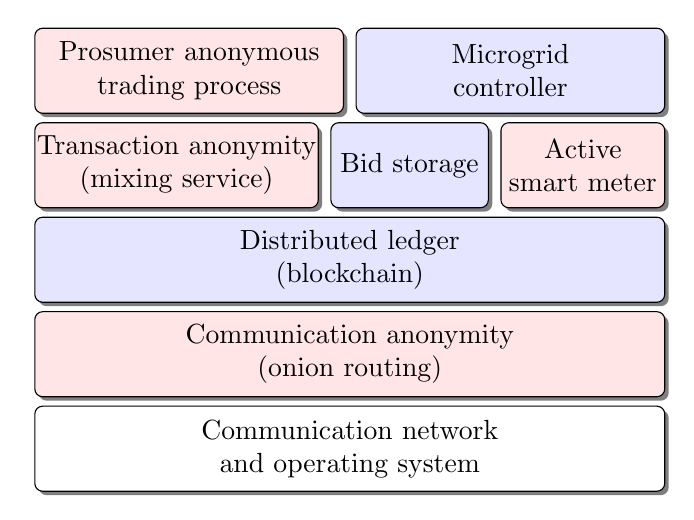
\begin{tikzpicture}[x=8cm, y=1.2cm,
  nodeStyle/.style={rounded corners=0.1cm, drop shadow={shadow xshift=0.05cm, shadow yshift=-0.05cm, fill=black}}
]
\draw [nodeStyle, fill=white]   (0, 0) rectangle    (1, 0.9) node [midway, align=center] {Communication network\\and operating system};

\draw [nodeStyle, fill=red!10]  (0, 1) rectangle    (1, 1.9) node [midway, align=center] {Communication anonymity\\(onion routing)};

\draw [nodeStyle, fill=blue!10] (0, 2) rectangle    (1, 2.9) node [midway, align=center] {Distributed ledger\\(blockchain)};

\draw [nodeStyle, fill=red!10]  (0,    3) rectangle (0.45, 3.9) node [midway, align=center] {Transaction anonymity\\(mixing service)};
\draw [nodeStyle, fill=blue!10] (0.47, 3) rectangle (0.72, 3.9) node [midway, align=center] {Bid storage};
\draw [nodeStyle, fill=red!10 ] (0.74, 3) rectangle (1,    3.9) node [midway, align=center] {Active\\smart meter};

\draw [nodeStyle, fill=red!10] (0,    4) rectangle (0.49, 4.9) node [midway, align=center] {Prosumer anonymous\\trading process};
\draw [nodeStyle, fill=blue!10] (0.51, 4) rectangle (1,    4.9) node [midway, align=center] {Microgrid\\controller};
\end{tikzpicture}
\caption{High-level architecture of the proposed solution. Components marked red are introduced to provide privacy in a safe and secure manner. Components marked in blue are typical elements of a decentralized transactive microgrid.}
\label{fig:softwareArchitecture}
\end{figure}

\begin{figure*}[h]
\center
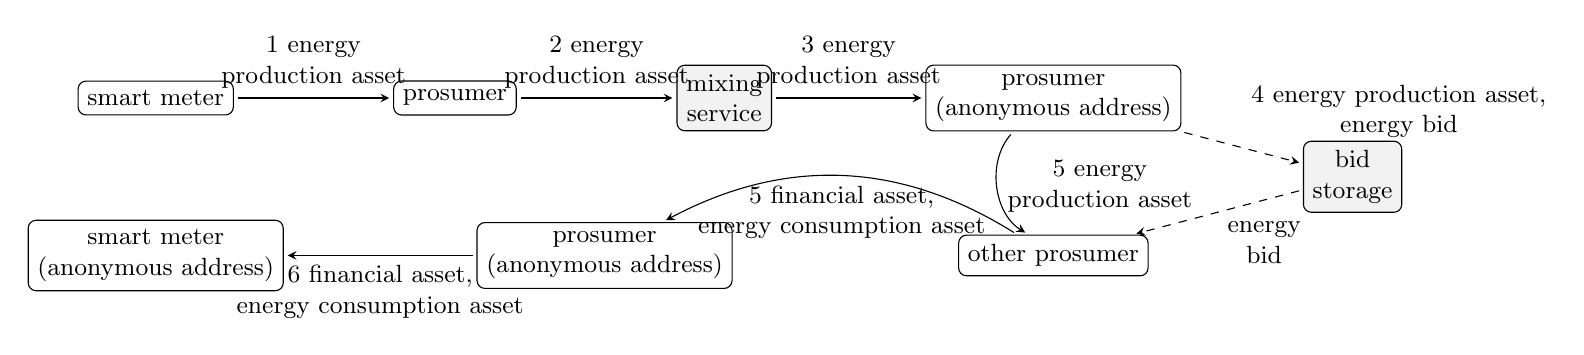
\begin{tikzpicture}[x=3.8cm, y=2cm, font=\small,
  system/.style={draw, align=center, rounded corners=0.1cm, fill=black!5},
  entity/.style={draw, align=center, rounded corners=0.1cm},
  asset/.style={midway, align=center},
  transfer/.style={->, >=stealth, shorten <=0.05cm, shorten >=0.05cm},
]
%\node[entity] (smartmeter) at (0.75, 0.5) {smart\\meter};
%\node[entity] (prosumer1) at (1.25, 1) {prosumer};
%\node[system] (mixing1) at (2, 1) {mixing\\service};
%\node[entity] (prosumer2) at (3, 1) {prosumer\\(alternative address)};
%\node[system] (bidstorage) at (4, 1) {bid\\storage};
%\node[entity] (partner) at (4, 0) {other prosumer};
%\node[entity] (prosumer3) at (3, 0) {prosumer\\(alternative address)};
%\node[system] (mixing2) at (2, 0) {mixing\\service};
%\node[entity] (prosumer4) at (1.25, 0) {prosumer};
\node[entity] (smartmeter) at (0, 1) {smart meter};
\node[entity] (prosumer1) at (1, 1) {prosumer};
\node[system] (mixing1) at (1.9, 1) {mixing\\service};
\node[entity] (prosumer2) at (3, 1) {prosumer\\(anonymous address)};
\node[system] (bidstorage) at (4, 0.5) {bid\\storage};
\node[entity] (partner) at (3, 0) {other prosumer};
\node[entity] (prosumer3) at (1.5, 0) {prosumer\\(anonymous address)};
\node[entity] (smartmeter2) at (0, 0) {smart meter\\(anonymous address)};

%\draw[transfer] (smartmeter) -- node [asset, above left] {energy\\production asset} (prosumer1);
%\draw[transfer] (prosumer1) -- node [asset, above] {energy\\production asset} (mixing1);
%\draw[transfer] (mixing1) -- node [asset, above] {energy\\production asset} (prosumer2);
%\draw[transfer, dashed] (prosumer2) -- node [asset, above] {energy production asset,\\energy bid} (bidstorage);
%\draw[transfer, dashed] (bidstorage) -- node [asset, right] {energy\\bid} (partner);
%\draw[transfer, bend right=15] (partner) to node [asset, below] {financial asset,\\energy\\consumption asset} (prosumer3);
%\draw[transfer, bend right=7.5] (prosumer2) to node [asset, above right] {energy\\prod. asset} (partner);
%\draw[transfer] (prosumer3) -- node [asset, below] {financial asset,\\
%energy consumption asset} (mixing2);
%\draw[transfer] (mixing2) -- node [asset, below] {financial asset,\\energy consumption asset} (prosumer4);
%\draw[transfer] (prosumer4) -- node [asset, below left] {financial\\asset} (smartmeter);

\draw[transfer] (smartmeter) -- node [asset, above] {\circled{1} energy\\production asset} (prosumer1);
\draw[transfer] (prosumer1) -- node [asset, above] {\circled{2} energy\\production asset} (mixing1);
\draw[transfer] (mixing1) -- node [asset, above] {\circled{3} energy\\production asset} (prosumer2);
\draw[transfer, dashed] (prosumer2) -- node [asset, above right] {\circled{4} energy production asset,\\energy bid} (bidstorage);
\draw[transfer, dashed] (bidstorage) -- node [asset, below right] {energy\\bid} (partner);
\draw[transfer, bend right=30] (partner) to node [asset, below] {\circled{5} financial asset,\\energy consumption asset} (prosumer3);
\draw[transfer, bend right=50] (prosumer2) to node [asset, right] {\circled{5} energy\\production asset} (partner);
\draw[transfer] (prosumer3) -- node [asset, below] {\circled{6} financial asset,\\
energy consumption asset} (smartmeter2);
\end{tikzpicture}
\caption{Simplified overview of the flow of assets from the perspective of a prosumer who sells energy. Note that in order to prevent de-anonymization, a prosumer should use multiple addresses and multiple rounds of mixing.}
\label{fig:sellFlow}
\end{figure*}

\subsection{Overview of the Trading Process}
We begin with a semi-formal description of the energy trading process from the prosumers' perspective.
In subsequent subsections, we will describe the assets, transactions, and services in our system in more detail.

First, consider a prosumer who would like to sell energy to another prosumer (this case is illustrated in Figure~\ref{fig:sellFlow}).
As its very first step, the prosumer obtains an \emph{energy production asset} from its smart meter.
An energy production asset represents a permission to sell a certain amount of energy, and it is used to enforce safety requirements.
If the prosumer has sufficient unsold production capacity, the smart meter creates and transfers a production asset to the prosumer using a \emph{smart meter transaction} \circled{1}, which is recorded on the distributed ledger.

At this point, the production asset can still be traced back to the prosumer since the ledger is public.
To achieve anonymity, the prosumer transfers the production asset to a \emph{mixing service} using an \emph{energy and financial transaction} \circled{2}, which is also recorded on the distributed ledger.
In turn, the mixing service transfers the production asset to an \emph{anonymous address} \circled{3}\todo{We should probably insert a good definition here for reader who are unfamiliar with blockchain transactions.}, which is randomly generated and controlled by the prosumer.
Since the mixing service transfers assets from multiple prosumers to multiple anonymous addresses at the same time, and the anonymous addresses were chosen at random by the prosumers, the assets cannot be traced back to the original prosumers after mixing.\footnote{Note that prosumers should divide their assets between multiple anonymous addresses; otherwise, each asset might be traced back to its prosumer based on the amount of energy that it contains.}

Now, the prosumer can engage in energy trading anonymously.
To find a trade partner, it can either post an \emph{energy bid} on the bid storage, or simply search the storage for an acceptable \emph{energy ask}.
To post an energy bid, the prosumer first proves to the storage service -- without revealing its original identity -- that it owns a production asset stored at an anonymous address.
It can then post the energy bid \circled{4}, which contains an anonymous communication address\footnote{We discuss communication anonymity later.}, a price, and a reference to the production asset.
If another prosumer, who would like to buy energy, finds the bid acceptable, it can contact the selling prosumer at the communication address given by the bid.

The seller and buyer can execute the trade by creating an energy and financial transaction together \circled{5}, and recording it on the ledger.
This transaction transfers the production asset from the seller to the buyer, and a \emph{financial asset} and an \emph{energy consumption asset} from the buyer to the seller.
A financial asset represents a certain amount of money, while a consumption asset represents a permission to buy a certain amount of energy, which is used to enforce safety requirements similarly to production assets.

Finally, the selling prosumer deposits the financial and consumption assets to its smart meter using an energy and financial transaction.
To ensure that the prosumer remains anonymous, it transfers the assets to an anonymous address that is randomly generated and controlled by the smart meter \circled{6}.
Once the smart meter has received the assets, it credits the financial amount to and deducts the energy amount from the prosumer, for billing purposes.
Note that in order to enforce safety requirements, the prosumer must always deposit the same amount of consumption assets as the amount of production assets obtained at the beginning; otherwise, unaccounted consumption assets might be used to trade excessive amounts.

Second, consider a prosumer who would like to buy energy from another prosumer.
Since the trading process is very similar to the case of the selling prosumer, we will discuss only the differences.
In the first step, the prosumer tries to obtain a financial asset and an energy consumption asset from its smart meter.
If the prosumer has the consumption capacity and good financial standing, the smart meter transfers the assets to the prosumer and adds the financial amount to the prosumer's bill.
After transferring the assets through a mixing service, the prosumer is ready to post an energy ask on the bid service.
To do so, it first proves the ownership of both the financial asset and the consumption asset to the service, and then posts the energy ask, which includes an anonymous communication address.
If a partner is found, the trade is executed as described before, the prosumer playing the role of the buyer.
Finally, the prosumer deposits the purchased energy production asset to the anonymous address of its smart meter,
which credits the energy amount to the prosumer, for billing purposes.
Note that if the prosumer has not used up the financial asset completely, then the remainder may also be deposited back to the smart meter.

\subsection{Timing}
The ability to specify points or intervals in time is crucial.
For example, control signals specify how the load should change at certain points in time, energy trades specify when energy will be consumed or produced, etc.
To facilitate processing signals and transactions, we divide time into fixed-length intervals, and specify points or periods in time using these discrete timesteps.
The length of the time interval is determined by mapping the timing assumptions of the power system to our platform.
%In our implementation, 
For example, the default length of the time interval may be 4 seconds, which corresponds to how frequently the control signal of the DSO typically changes.

\subsection{Transactions}

In the previous subsection, we gave an overview of how transactions are used in the trading process to transfer various assets.
Here, we detail the format of these transactions, and the rules that they have to satisfy to be valid and recorded on the ledger.
We also introduce and detail the format of regulatory transactions, which the DSO uses to regulate the microgrid.

\subsubsection{Timing}

The ability to specify points or intervals in time is crucial.
For example, control signals specify how the microgrid load should change at certain points in time, energy trades specify when energy will be consumed or produced, etc.
To facilitate processing signals and transactions, we divide time into fixed-length intervals, and specify points or periods in time using these discrete timesteps.
The length of the time interval is determined based on the timing assumptions of the physical power system.
For example, the default length of the time interval may be 4 seconds, which corresponds to how frequently the control signal of the DSO typically changes.
\Abhishek{We need to add citation here. I will add that tomorrow.}
\Abhishek{What about the deadline within which the transactions should finish? Do we need to say anything here?}
\Aron{Ideally, we should discuss the timing constraints of the ledger (probably when we introduce it), but we would first need to make space for this discussion.}

\subsubsection{Assets}

Before we can discuss transactions, we must define the format of three assets that these transactions may transfer.
First, an \emph{energy production asset} (EPA) is defined by
\begin{compactitem}
\item \field{power}: non-negative amount of power to produced (for example, measured in watts),
\item \field{start}: first time interval in which energy is to be produced,
\item \field{end}: last time interval in which energy is to be produced.
\end{compactitem}
Second, an \emph{energy consumption asset} (ECA) is defined by the same fields; however, for this asset, the fields define energy consumption instead of production.
Finally, a \emph{financial asset} (FA) is defined by a single non-negative number \field{amount}, which can be denominated in either a fiat currency (e.g., US dollars) or a cryptocurrency.

\subsubsection{Energy and Financial Transactions}

Energy and financial transactions transfer energy and financial assets from one address to another.
Prosumers use these transactions for multiple purposes: to trade energy by exchanging assets with other prosumers, to prove to the bid storage that they have production or consumption capacity, to hide their identity by transferring assets to and from mixing services, and to deposit assets at their smart meter.
%
An energy and financial transaction contains the following fields:
\begin{compactitem}
\item \field{EPA\_in}: list of EPA inputs, each of which is defined by
\begin{itemize}[leftmargin=0.5em,nosep]
\item \field{out}: reference to an EPA output of a previous transaction,
\item \field{sig}: signature for referenced output,
\end{itemize}
\item \field{ECA\_in}: list of ECA inputs, each of which is defined by
\begin{itemize}[leftmargin=0.5em,nosep]
\item \field{out}: reference to an ECA output of a previous transaction,
\item \field{sig}: signature for referenced output,
\end{itemize}
\item \field{FA\_in}: list of FA inputs, each of which is defined by
\begin{itemize}[leftmargin=0.5em,nosep]
\item \field{out}: reference to an FA output of a previous transaction,
\item \field{sig}: signature for referenced output,
\end{itemize}
\item \field{EPA\_out}: list of EPA outputs, each of which is defined by
\begin{itemize}[leftmargin=0.5em,nosep]
\item \field{EPA}: an energy production asset,
\item \field{address}: address to which EPA is transferred,
\end{itemize}
\item \field{ECA\_out}: list of ECA outputs, each of which is defined by
\begin{itemize}[leftmargin=0.5em,nosep]
\item \field{EPA}: an energy consumption asset,
\item \field{address}: address to which ECA is transferred,
\end{itemize}
\item \field{FA\_out}: list of FA outputs, each of which is defined by
\begin{itemize}[leftmargin=0.5em,nosep]
\item \field{EPA}: a financial asset,
\item \field{address}: address to which FA is transferred,
\end{itemize}
\end{compactitem}
This transaction transfers the assets specified in the input lists to the addresses specified in the output lists. 
Note that assets may be divided or combined, as the input and output lists may differ in length.

An energy and financial transaction is valid (and can be recorded on the ledger) if the following three conditions hold.
\begin{itemize}[noitemsep,topsep=-\parskip]
\item None of the outputs referenced by the inputs have been spent by a transaction that has been recorded on the ledger.
\item All of the signatures are valid, which ensures that only the current owner can transfer an asset.
\item For each asset type (and for each timestep), the sum of inputs and outputs is equal.
For example, in the case of energy production assets, the condition is
\begin{align*}
& \forall t: \sum_{\substack{out \,\in\, \field{EPA\_out}:\\out.\field{EPA}.\field{start} \leq t \leq out.\field{EPA}.\field{end}}} out.\field{EPA}.\field{power} \nonumber \\
& = \sum_{\substack{in \,\in\, \field{EPA\_in}:\\in.\field{out}.\field{EPA}.\field{start} \leq t \leq in.\field{out}.\field{EPA}.\field{end}}} in.\field{out}.\field{EPA}.\field{power}  .
%
%& \forall t: \sum_{out \in \field{EPA\_out}} out.\field{EPA}.\field{power} \cdot 1_{\left\{out.\field{EPA}.\field{start} \leq t \leq out.\field{EPA}.\field{end}\right\}} \nonumber \\
%& = \sum_{in \in \field{EPA\_in}} in.\field{out}.\field{EPA}.\field{power} \cdot 1_{\left\{in.\field{out}.\field{EPA}.\field{start} \leq t \leq in.\field{out}.\field{EPA}.\field{end}\right\}} ,
\end{align*}
%where $1_x$ is equal to $1$ if $x$ is true, and it is $0$ otherwise.
%\begin{equation}
%\forall t: \sum_{out \in \left\{out' \middle| out' \in \text{ EPA outputs} \wedge out'.EPA.start \leq t \leq out'.EPA.end\right\}} out.EPA.Power = \sum_{in \in \left\{in' \middle| in' \in \text{ EPA inputs} \wedge in'.EPA.start \leq t \leq in'.EPA.end\right\}} in.EPA.Power .
%\end{equation}
The conditions for consumption and financial assets can be described formally in similar ways.
\end{itemize}
%If a transaction submitted to the ledger is valid, it will be permanently recorded.

\subsubsection{Smart-Meter Transactions}

Prosumers use smart-meter transactions to withdraw energy and financial assets from their own smart meters, before they engage in trading.
%
A transaction contains the following fields:
\begin{compactitem}
\item \field{EPA\_out}: list of EPA outputs (see above),
\item \field{ECA\_out}: list of ECA outputs (see above),
\item \field{FA\_out}: list of FA outputs (see above),
\item \field{id}: smart meter's identifier,
\item \field{sig}: smart meter's signature over the transaction.
\end{compactitem}
This transaction creates and transfers the assets to the prosumer's addresses, which are specified in the output lists.

The smart meter signs the transaction only if the prosumer is allowed to withdraw these assets.
More specifically, the amount of withdrawn assets can never exceed certain limits that are set by the DSO.
For example, in the case of EPA, the following condition must be satisfied for prosumer $i$:
\begin{equation}
\forall t: \sum_{tr \,\in\, \field{TR}_i} \sum_{\substack{out \,\in\, tr.\field{EPA\_out}:\\out.\field{EPA}.\field{start} \leq t \leq out.\field{EPA}.\field{end}}} out.\field{EPA}.\field{power} < \field{MAXEPA}_i ,
\end{equation}
where $\field{TR}_i$ is the set of smart-meter transactions recorded for prosumer $i$ and $\field{MAXEPA}_i$ is the withdrawal limit.
The condition for consumption assets is similar, based on a limit $\field{MAXECA}_i$.
For financial assets, the smart meter takes into account the amounts withdrawn and deposited, as well as the outside bill payments to the DSO.

\Aron{To address malfunctioning or compromised smart meters, we could also impose a limit on withdrawals.}
A transaction is valid if the following two conditions hold.
\begin{itemize}[noitemsep,topsep=-\parskip]
\item The smart meter identified in the transaction has been authorized by a regulatory transaction that was previously recorded on the ledger.
\item The smart meter's signature is valid (for public key, see regulatory transactions).
\end{itemize}

\subsubsection{Regulatory Transactions}

The DSO uses regulatory transactions for two purposes: to manage the set of authorized smart meters and to change the price policy.
%First, to change the set of smart meters that are authorized to sign transactions, the DSO authorizes or bans individual smart meters.
First, whenever a new smart meter is installed, the DSO notifies the microgrid by authorizing the device using a regulatory transaction.
Similarly, whenever a smart meter is deactivated (e.g., because service is stopped or the device is believed to be malfunctioning or compromised), the DSO notifies the microgrid by banning the device.
Second, to influence microgrid load, the DSO can set a price policy, which includes a price at which prosumer may buy energy from the DSO and a price at which they may sell energy to the DSO.

A regulatory transactions contain the following fields:
\begin{compactitem}
\item \field{authorize}: list of smart meters to be authorized, each of which is defined by
\begin{compactitem}
\item \field{id}: identifier of the smart meter,
\item \field{pubkey}: public key of the smart meter,
\end{compactitem}
\item \field{ban}: list of identifiers of smart meters to be banned, 
\item \field{priceConsumption}: price at which DSO sells energy,
\item \field{priceProduction}: price at which DSO buys energy,
\item \field{time}: timestep after which authorizations, bans, and price changes should take effect,
\item \field{sig}: DSO's signature over the transaction.
\end{compactitem}

A regulatory transaction of this type is valid if %the following two conditions hold:
%\begin{compactitem}
%\item 
\field{timestep} is not in the past and % specified in the transaction is in the future.
%\item 
the DSO's signature is valid.
%\end{compactitem}
%
The active prices for timestep $t$ are given by the last regulatory transaction recorded on the ledger whose \field{time} is less than $t$.
Similarly, regulatory transactions that are recorded on the ledger later override the authorizations and bans of earlier transactions.



\subsection{Services}

In this subsection, we describe the various services that are implemented in our system. %on which transactions are built and which build on transactions.
We have already discussed the distributed ledger, which permanently stores valid transactions.
Now, we will introduce anonymous communication service, mixing service for transaction anonymity, anonymous bid storage, and smart-meter based billing.\Aron{Revise list based on final organization!}

\subsubsection{Communication Anonymity}
Firstly, we must provide an anonymous communication layer, on which we can build all the other services in our system.
Without this communication layer, transactions and bids could be easily de-anonymized based on their sources' network identifiers (e.g., IP or MAC addresses).

We can employ well-known and widely used techniques for anonymous communication, such as \emph{onion routing}~\cite{reed1998anonymous}.
To build an onion network, the smart meters, prosumers, and other devices can act as onion routers, and the list of onion routers in a microgrid can be published on the ledger.
In practice, this service can built on 
%In our first implementation, we can use
 the free and open-source Tor software with private Directory Authorities.
In this case, anonymous communication addresses in bids and asks correspond to public-keys that identify Tor hidden services.
% ritter.vg: "run your own tor network"
% https://ritter.vg/blog-run_your_own_tor_network.html

\subsubsection{Transaction Anonymity}
Communication anonymity is necessary for anonymous trading, but it is not sufficient: if prosumers used their own accounts to transfer assets, trades would not be anonymous.
Fortunately, most distributed ledgers allow users to easily generate new addresses\footnote{The usage of the term \emph{address} varies between distributed ledgers, but our system could be implemented using any popular ledger, such as Bitcoin and Ethereum. 
Specifically, we use the term address to denote a possible destination for asset transfers. 
Assets transferred to an address can be used only by someone who knows the private key of the address (typically, the one who generated the address).} 
at random.
Since these addresses are generated randomly, they are anonymous in the sense that no one can tell who generated them.
However, if prosumers simply transferred assets to these addresses, they could be easily de-anonymized by tracing the assets back to the prosumers.

To prevent this, prosumers transfer assets to their anonymous addresses through a \emph{mixing service}. 
The mixing service prevents tracing the assets back to their original owners by mixing together multiple incoming transfers and multiple outgoing transfers, thereby hiding the connections between the prosumers and the anonymous addresses.
In practice, a mixing service can be implemented using multiple approaches.
The simplest one is to use a \emph{trusted third party}, called a cryptocurrency tumbler, which can receive and send assets.
However, anonymity in this case depends on the trustworthiness and reliability of the third party, who could easily de-anonymize the addresses.
A more secure approach is to used decentralized protocols, such as CoinShuffle~\cite{ruffing2014coinshuffle} or Xim~\cite{bissias2014sybil}.
These protocols enable participants to mix assets with each other, thereby eliminating the need for a trusted third party, which would constitute a single point of failure.
Some newer cryptocurrencies, such as Zerocoin~\cite{miers2013zerocoin},  provide built-in mixing services, which are often based on cryptographic principles and proofs.

\begin{comment}
We must provide prosumers with the ability to create and publish transactions anonymously.
More specifically, prosumers should be able to purchase or sell energy without revealing their identity; however, these transaction must also be verifiable and enforceable.

We may achieve this goal using multiple approaches for blockchain transaction anonymity:
\begin{itemize}
\item Mixing services (also known as tumblers) mix potentially identifiable assets on a blockchain with others, thereby preventing tracing individual assets back to their original source. 
In our case, assets to be mixed include virtual balances of fiat currencies as well as energy production and consumption.
\item Cryptographic anonymity for transactions is provided, for example, by Zerocoin~\cite{miers2013zerocoin}. Similarly to mixing service, Zerocoin can prevent tracing assets on a blockchain.
\end{itemize}
Using the above techniques, we can enable prosumers to trade energy anonymously (i.e., without revealing their true identities), but at the same time prevent them from altering their energy or financial balances without a valid transaction.

However, we must also ensure that 1) smart meters know the amount of energy purchased or sold by their prosumer and 2) prosumers cannot purchase or sell more energy than their capacity.
To satisfy both of these constraints, all energy trades must start with the prosumer withdrawing a certain amount of energy production or consumption from its smart meter:
\begin{itemize}
\item If a prosumer wishes to sell energy, it must first withdraw an energy asset from its smart meter using a blockchain transaction.
This transaction must be signed by the smart meter, which enables the smart meter to 1) keep track of the amount of energy traded by the prosumer as well as to 2) enforce safety requirements by limiting the amount of energy that can be withdrawn.
\item If a prosumer wishes to buy energy, it must first withdraw an energy consumption asset from its smart meter in a way similar to withdrawing an energy production asset.
\end{itemize}
\end{comment}

\subsubsection{Bidding Anonymity}
Finally, we must provide prosumers with the ability to post energy bids and asks anonymously.
To this end, we create a storage for anonymous bids that is readable by all the prosumers in the microgrid.
Any prosumer may submit a bid to this storage; however, in order to do so, they must provide a zero-knowledge proof of owning the assets that are to be traded:
\begin{itemize}
\item To submit an energy sell bid, the prosumer must prove that it owns an energy production asset on the chain.
\item To submit an energy buy bid, the prosumer must prove that it own an energy consumption asset as well as financial assets on the chain.
\end{itemize}

\subsubsection{Billing}

The energy consumption balance $E_i^t$ of prosumer $i$ in timeslot~$t$ is
\begin{align*}
E_i^t = & \hphantom{+} \text{measured consumption} - \text{measured production} \\
 & + \text{EPA deposited by $i$} - \text{EPA withdrawn by $i$} .
\end{align*}
Notice that energy consumption assets are not necessary for billing, they are only used to enforce safety requirements.

The financial balance $F_i^t$ of prosumer $i$ in timeslot $t$, which is to be paid by the prosumer to the DSO, is
\begin{align*}
F_i^t = & \hphantom{+} \text{FA deposited by $i$ in $t$} - \text{FA withdrawn by $i$ in $t$} \\
 & + \begin{cases}
E_i^t \cdot \field{priceProduction} & \text{ if } E_i^t < 0 \\
- E_i^t \cdot \field{priceConsumption} & \text{ otherwise.} 
\end{cases}
\end{align*}

\TODO{discussion of microgrid control based on bids and trades? (update subsubsection title)}




\subsection{Smart Contract}
\label{sec:smartcontract}

We implement a smart contract that can (1) verify whether a solution is feasible and (2) compute the value of the objective function for a feasible solution.
Compared to finding an optimal solution, these operations are computationally inexpensive, and they can easily be performed on a blockchain-based decentralized platform. Thus, we implement a smart contract that provides the following functionality:
\begin{itemize}
\item Solutions may be submitted to the contract at any time during the solving phase. 
The contract verifies the feasibility of each submitted solution, and if the solution is feasible, then it computes the value of the objective function.
The contract always keeps track of the best feasible solution submitted so far, which we call the \emph{candidate solution}.
\item At the end of the solving phase, the contract finalizes resource assignments for the cycle based on the candidate solution. If no solution has been submitted to the contract, then an empty allocation is used as a solution, which is always feasible but attains zero objective. % which might be the case right after the trading system has been launched then the finalization event does not return any solution.
%\item Upon finalization, the contract must notify providers and consumers about finalized assignments. 
%This can be done using the event filter mechanisms provided by blockchains like Ethereuem. \cite{ref}.
\end{itemize}

This simple functionality achieves a high level of security and reliability.
Firstly, it is clear that an adversary cannot force the contract to finalize assignments based on an incorrect (i.e., infeasible) solution since such a solution would be rejected.
Similarly, an adversary cannot force the contract to choose an inferior solution instead of a superior one.
In sum, the only action available to the adversary is proposing a superior feasible solution, which would actually improve the transactive management platform.

%\Aron{This paragraph should be omitted (and included in the Industrial Informatics paper).}
%The contract is also reliable and can tolerate temporary disruptions in the solver or the communication network. As the sets of offers can only grow over time, the contract can use a candidate solution submitted during time interval $t$ to finalize assignments in any subsequent time interval $\tau > t$.
%In fact, without receiving new solutions, the difference between the amount of finalized assignments and the optimum will increase only gradually:
%since the earlier candidate solution can specify assignments for any future time interval,
%the difference is only due to the offers that have been posted since the solution was found and submitted.

%\subsection{Correct-by-Construction Design of the Smart Contract}
To ensure that the smart-contract code is correct-by-construction~\cite{sifakis2013RSD}, we use the formal design environment FSolidM~\cite{mavridou2018designing} to design and generate the Solidity code of the smart contract. FSolidM allows designing Ethereum smart contracts as Labelled Transition Systems (LTS) with formal semantics. Each LTS can then be given to the NuSMV model checker~\cite{cimatti2002nusmv} to verify liveness, deadlock-freedom, and safety properties, which can capture important security concerns. % and vulnerabilities. 


\begin{figure}[t]
\centering
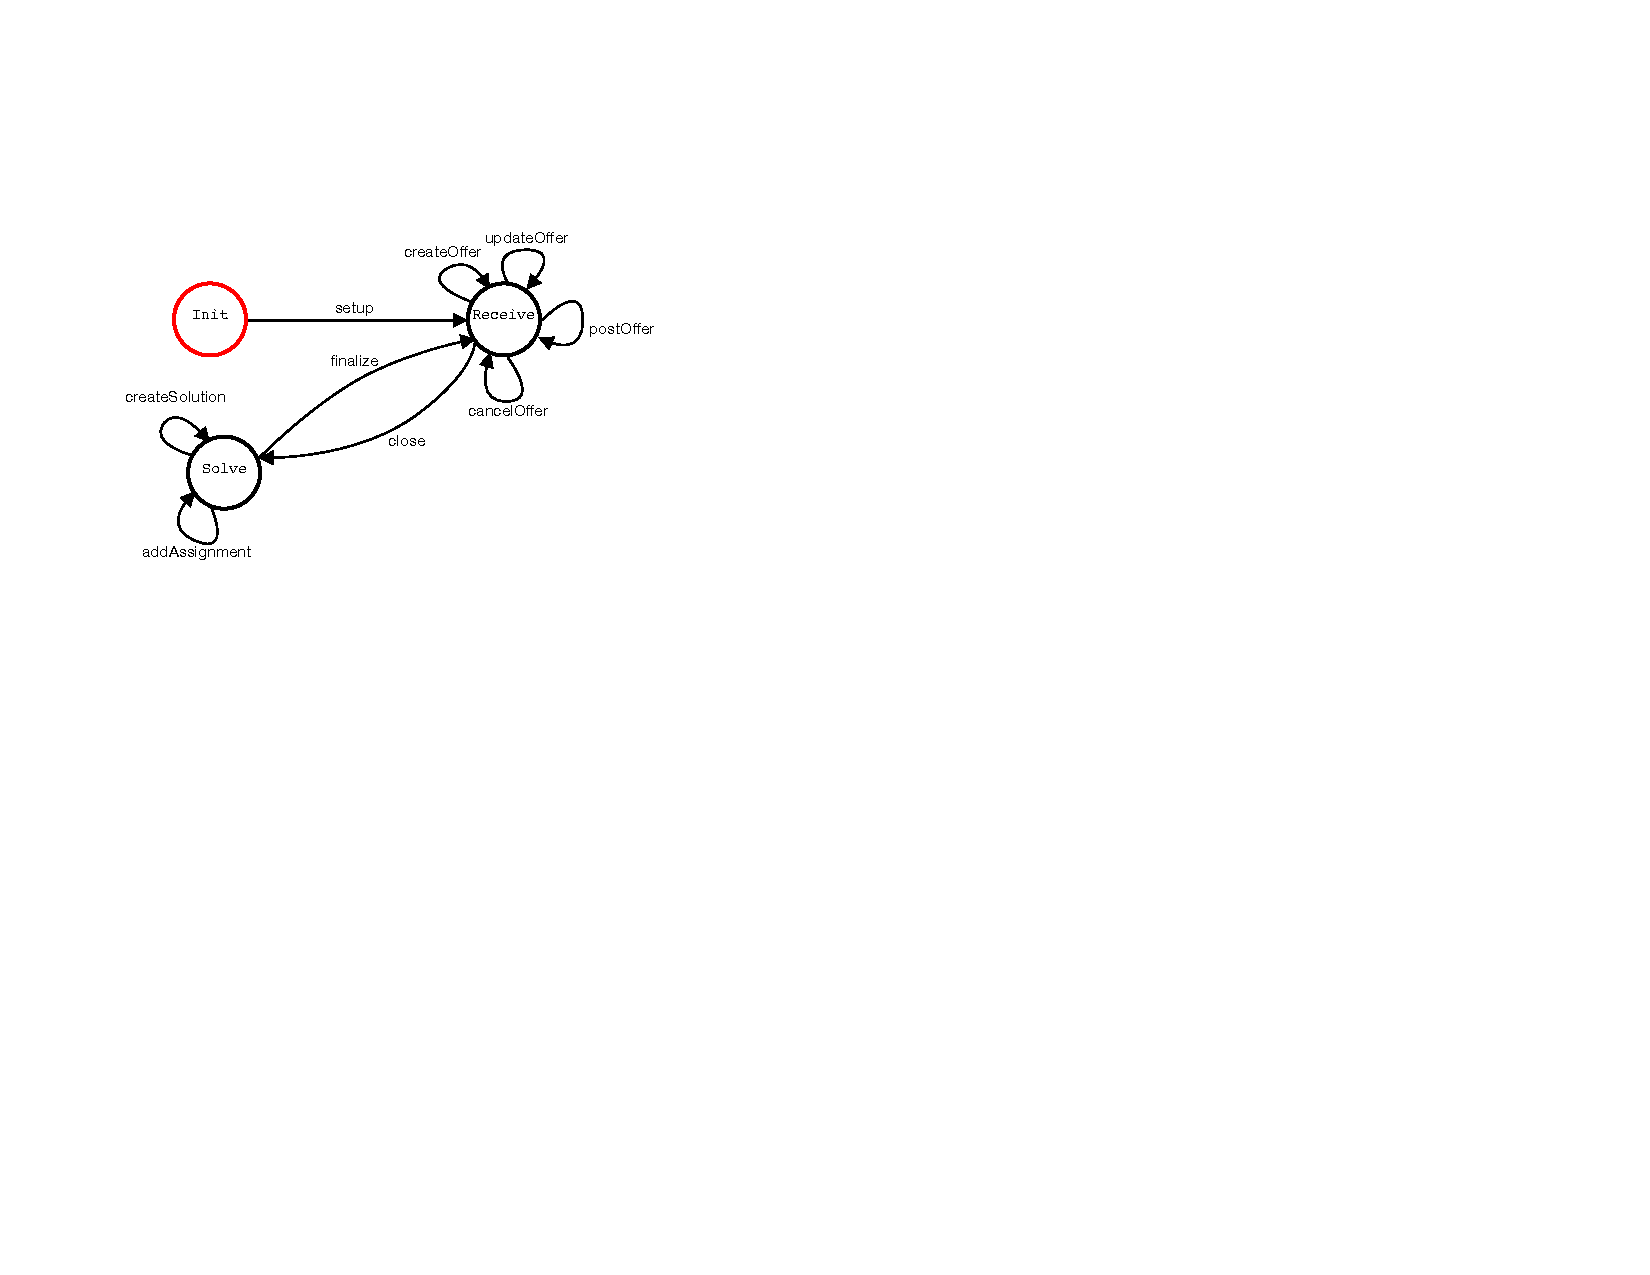
\includegraphics[width=0.8\columnwidth]{ResourceAllocationFSM.pdf}
\caption{FSolidM model of the \Platform smart contract.}
\label{fig:FSM}
\end{figure}

%\ad{Aron - please explain all the states of the smart contract here. The state machine diagram should be updated as well. please describe the mapping structure - how types are mapped in the smart contract here as well.}
%\Aron{What do you mean by mapping structure?}
%\Anastasia{I have updated the LTS figure and the description. }

In Figure~\ref{fig:FSM}, we present the LTS representation of the transactive-platform smart contract, designed with FSolidM. The contract has three states:\footnote{Generated smart-contract code is not included in the paper because of space constraints. However, interested readers can view the code at \texttt{\url{https://github.com/visor-vu/transaction-management-platform}}}
\begin{itemize}[noitemsep, topsep=0pt, leftmargin=1em]
    \item \texttt{Init}, in which the contract has been deployed but  not been initialized. Before the contract can be used, it must be initialized (i.e., numerical parameters must be set~up).
    \item \texttt{Receive}, which corresponds to the \emph{offering} phase of a cycle (see Section~\ref{sec:scheduling}).
    In this state, prosumers may post (or cancel) their offers.
    \item \texttt{Solve}, which corresponds to the \emph{solving} phase of a cycle (see Section~\ref{sec:scheduling}). In this state, solvers may submit solutions (i.e., resource allocations) based on the posted (but not cancelled) offers.
\end{itemize}

In FSolidM, smart-contract functions are modeled as LTS transitions. Note that by design, each function may be executed only if the contract is in the origin state of the corresponding transition.
Our smart contract  has the following transitions (after the name of each transition, we list the function parameters):
\begin{itemize}[leftmargin=1em, noitemsep]
    \item from state \texttt{Init}:
    \begin{itemize}[noitemsep, leftmargin=0.5em]
        \item \texttt{setup(uint64 numTypes, uint64 precision, uint64 maxQuantity)}: initializes a contract with numerical parameter values, setting up the number of resource types, the arithmetic precision for calculations, and the maximum quantity that may be offered; upon execution, the contract transitions to state \texttt{Receive}.
    \end{itemize}
    \item from state \texttt{Receive}:
    \begin{itemize}[noitemsep, leftmargin=0.5em]
        \item \texttt{createOffer(bool providing, uint64 misc))}: creates a blank offer (belonging to the prosumer invoking this transition) within the smart contract; parameter \texttt{providing} is true for providers and false for consumers, parameter \texttt{misc} is an arbitrary value that prosumers may use for their own purposes (e.g., to distinguish between their own offers); emits an \texttt{OfferCreated} event.
        \item \texttt{updateOffer(uint64 ID, uint64 resourceType, uint64 quantity, uint64 value)}: sets quantity and value for a resource type in an existing  offer (identified by the \texttt{ID} given in the \texttt{OfferCreated} event); may be invoked only by the entity that created the offer, and only if the offer exists but has not been posted yet; emits an \texttt{OfferUpdated} event.
        \item \texttt{postOffer(uint64 ID)}: posts an existing offer, enabling solvers to include this offer in a solution; may be invoked only by the entity that created the offer; emits an \texttt{OfferPosted} event.
        \item \texttt{cancelOffer(uint64 ID)}: cancels (i.e., ``unposts'') an offer, forbidding solvers from including this offer in a solution; may be invoked only by the entity that created the offer; emits an \texttt{OfferCanceled} event.
        \item \texttt{close()}: protected by a  guard condition on time, which prevents the execution of this transition before the offering phase of the current cycle ends; transitions to state \texttt{Solve}; emits a \texttt{Closed} event.
    \end{itemize}
    \item from state \texttt{Solve}:
    \begin{itemize}[noitemsep, leftmargin=0.5em]
        \item \texttt{createSolution(uint64 misc)}: creates a new, empty solution (i.e., resource allocation) within the smart contract; parameter \texttt{misc} is an arbitrary value that solvers may use for their own purposes (e.g., to distinguish between their own solutions); emits a \texttt{SolutionCreated} event.
        \item \texttt{addAssignment(uint64 ID, uint64 providingOfferID, uint64 consumingOfferID, uint64 resourceType, uint64 quantity, uint64 value)}: adds a resource assignment to an existing solution (identified by the \texttt{ID} given in the \texttt{SolutionCreated} event); may be invoked only by the entity that created the solution; checks a number of constraints ensuring that the solution remains valid if this assignment is added; emits an \texttt{AssignmentAdded} event.
        \item \texttt{finalize()}: selects the best solution and finalizes it by emitting an \texttt{AssignmentFinalized} event for each assignment in the solution; protected by a guard condition on time, which prevents the execution of this transition before the solving phase of the current cycle ends; transitions to state \texttt{Receive}.
    \end{itemize}
\end{itemize}
Notice that posting an offer and submitting a solution require at least three and two function calls, respectively.
The reason for dividing these operations into multiple functions is to ensure that the computational costs of these functions are constant.
Otherwise, posting a complex offer or submitting a complex solution could be infeasible due to large computational costs, which could exceed the gas limit.\footnote{In Ethereum, each transaction is allowed to consume only a limited amount of gas, which corresponds to the computational and storage cost of executing the transaction.}



% \begin{lstlisting}[language=Solidity, caption=Extract of the Generated Smart Contract. Full contract is available at \url{https://github.com/visor-vu/transaction-management-platform}. ,label={lst:finalize}]
% pragma solidity ^0.4.19;
% contract SolidWorx {     
%     function setup(...) public {
%         //setup SolidWorx to be used with a fixed type of resources. 
%     }
%     //This is the syntax of an offer.
%     struct Offer {
%         bool providing; 
%         // true: providing offer
%         // false: consumption offer
%         uint64 prosumer; 
%         bool posted;
%         mapping(uint64 => uint64) quantity;
%         mapping(uint64 => uint64) value;
%     }
%     //syntax of an Assignment
%     struct Assignment {
%         uint64 providingOfferID;
%         uint64 consumingOfferID;
%         uint64 resourceType;
%         uint64 quantity;
%         uint64 value;
%     }
%     //A solution contains many assignments.
%     struct Solution {
%         mapping(uint64 => Assignment) assignments;
%         uint64 numAssignments;
%         uint64 objective;
%         mapping(uint64 => uint256) allocated;     
%     }
%     function createOffer(bool providing, uint64 misc, uint64 prosumer) public {
%         ...
%     }
%     function updateOffer(uint64 ID, uint64 resourceType, uint64 quantity, uint64 value) public {
%         ...
%     }
%     function postOffer(uint64 ID) public {
%         ...
%     }
%     function cancelOffer(uint64 ID) public {
%         ...
%     }
%     ...
%     function createSolution(uint64 misc) public {
%         ...
%     }
%     function addAssignment(...) public {
%         ...
%     }
%     function finalize() public {
%         ...
%     }
% }
% \end{lstlisting}

%Listing \ref{lst:finalize} presents the generated API and the guards for the smart contract in \Platform. 




%\subsection{Operation Workflow }

\begin{figure}[t]
    \centering
    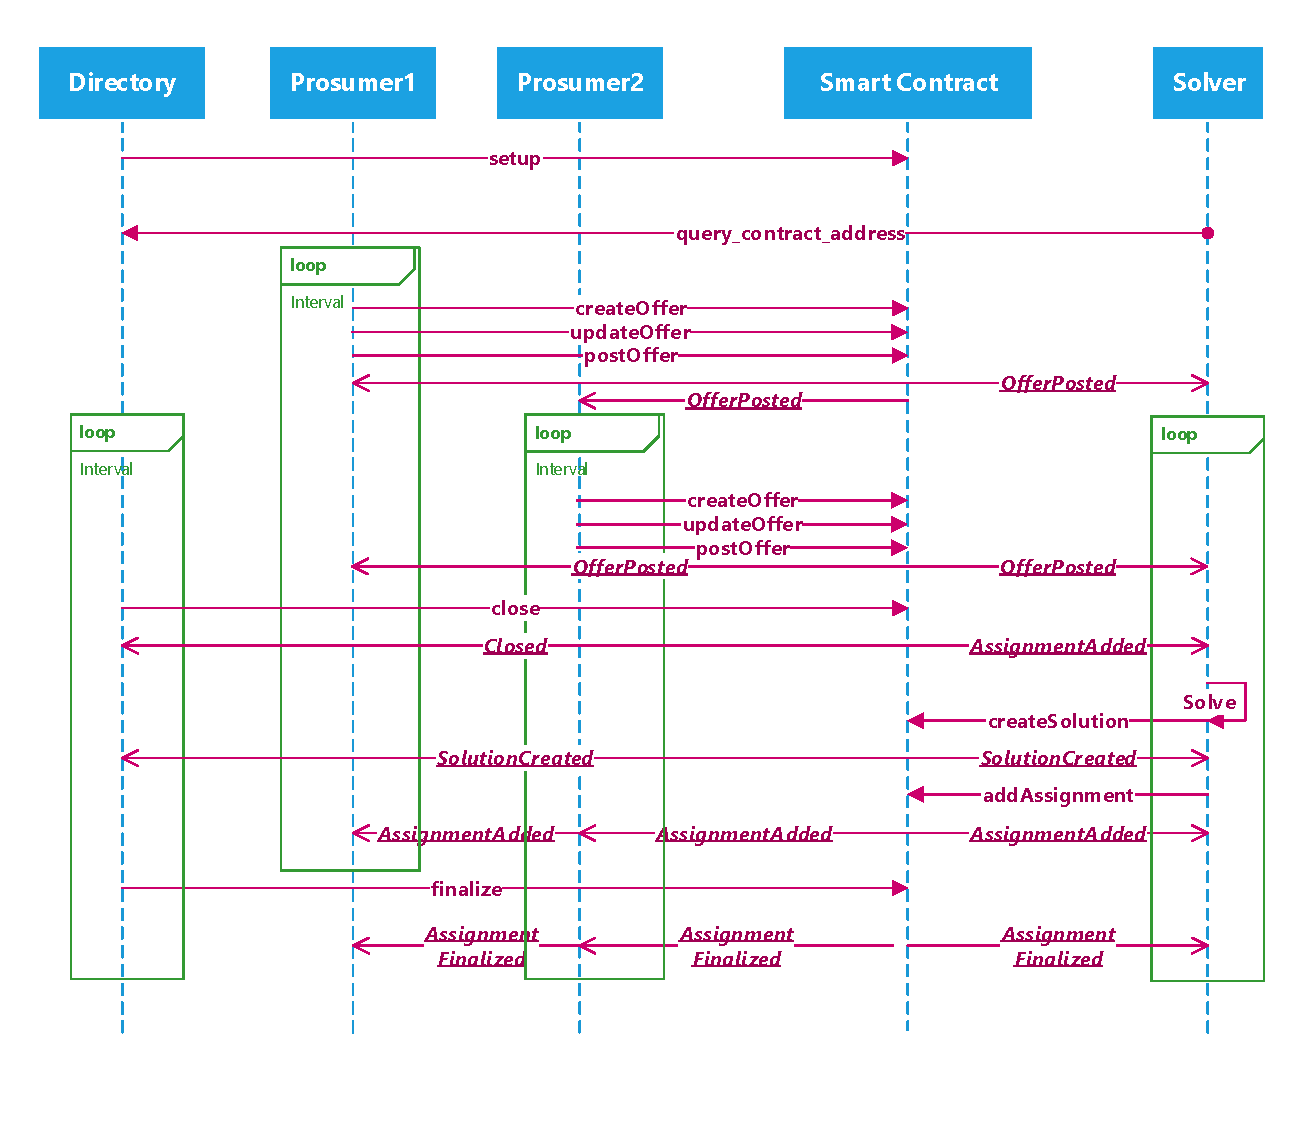
\includegraphics[width=\columnwidth]{Workflow.pdf}
    \caption{A possible sequence of operations in \Platform. Underlined text denotes events emitted by the smart contract. Some events, such as \texttt{OfferUpdated}, are omitted for simplicity. %The offers can be updated by a prosumer before they are marked as posted. 
    %See Listing \ref{lst:finalize} for the API.} % Prosumers and Solvers use the directory to find one of the miner nodes running the smart contract. They then connect to the  mining node.
    }
    \vspace{-0.1in}
    \label{fig:workflow}
\end{figure}

 A typical sequence of function calls and events in \Platform is shown in Figure \ref{fig:workflow}.


%\subsection{Workflow}
%\label{sec:analysis}
%\label{sec:workflow}
% api and sequence

\begin{figure}
    \centering
    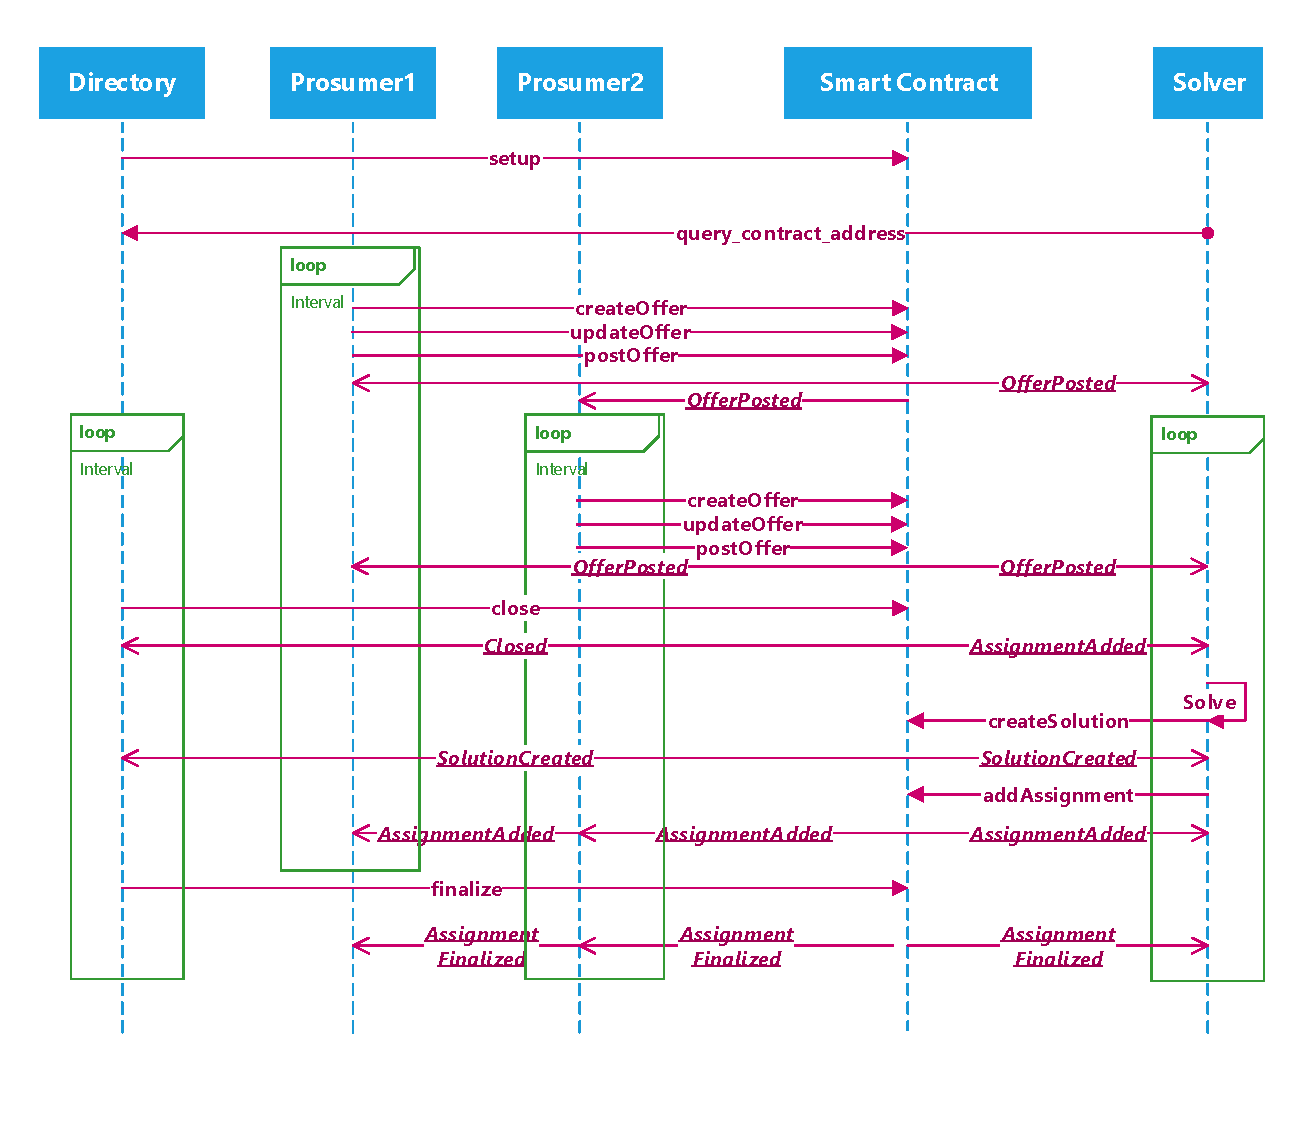
\includegraphics[width=\columnwidth]{Workflow.pdf}
    \caption{Sequence of operations in the transaction management platform.} % Prosumers and Solvers use the directory to find one of the miner nodes running the smart contract. They then connect to the  mining node.}
    \label{fig:workflow}
\end{figure}


\Aron{The figure has not much to do with the current platform. Key functions are missing, and non-existing functions are shown. Needs to be remove or updated!}
\Aron{What is the point of this subsection? This needs to be made clear at the beginning.}
Figure \ref{fig:workflow} describes the workflow of activity in this transaction management platform.  The specific operations in this workflow are described below. Note that the events in this workflow can arrive out of order at the smart contract. %For example, a consumer can request a resource from a time interval that has already been finalized by the smart contract. However, those consumption offers will be rejected.

\begin{itemize}[leftmargin=*]
\setlength{\itemsep}{0pt}%
    \setlength{\topsep}{0pt} 
    \setlength{\partopsep}{0pt}
    \setlength{\parsep}{0pt}
    \setlength{\parskip}{0pt}%
\item Deploying the contract \texttt{(bytecode)}\Aron{Writing ``deployContract'' in the figure suggests that there is a function named ``deployContract'' in the smart contract or the blockchain, which is not true.}: 
Blockchain transaction submitted by a directory actor. \Aron{Directory has not been mentioned in the text before!} The transaction deploys the smart contract, making it available for all participants to use. The blockchain returns the address of the deployed contract.\Aron{This is kind of obvious.}
\item \texttt{Connect}: \Aron{This is practically just establishing a TCP connection. Why do we mention this?!} Any new participant first connects to the directory. The directory can run an optional mixing service\Aron{Anonymization needs to be discussed more detail or omitted.}, providing the participants with an anonymous identifier.
\item \texttt{query\_contract\_address}:  This is an off-blockchain communication between participants and the directory, which returns the address of the smart contract. 
\item \texttt{registerProsumer(uint64 prosumer)}: \Aron{Remove this! It was not listed in the contract (see FSolidM section), and it has not been implemented.} Each prosumer registers with the smart contract, providing an anonymous identifier.
\item \texttt{ProsumerRegistered}: \Aron{Again, what is this doing here? There is nothing like this in the platform.} Event broadcast by the smart contract, notifying prosumers that they have registered. 
\item \texttt{postOffer(assetID, price)}: \Aron{Fuction signatures are all wrong...} smart contract function called by a prosumer, publicly posting an offer to produce or consume a resource. The resource type is encoded in the assetID and checked by the smart contract.
\item \texttt{OfferPosted(offerID, assetID, price)}: event broadcast by the smart contract, notifying solvers that an offer was posted.
%\item \texttt{Solve} : Once offers have been posted the Solver begins solving for potential matchings of the offers of which it has been notified. \Aron{This is not an interaction, so it should not be on this list. Further, we don't assume anything about solvers, so we really shouldn't discuss their internal working here.}
\item \texttt{createSolution(uint64 solverID)}: The Solver sends a request to the smart contract to tell it that a new solution has been found..
\item \texttt{SolutionCreated}: event broadcast by the smart contract, notifying the solver that it can submit the trades that constitute the new solution.
\item \texttt{addAssignment(uint64 solutionID, uint64 sellerID, uint64 buyerID, uint64 time, uint64 power)}: smart contract function called by the solver, which posts the trades to the solution created previously on the blockchain. As the trades are added the smart contract verifies that each is a valid trade and does not violate any of the system constraints.
\item \texttt{AssignmentAdded}: An event broadcast by the smart contract notifying the solver and the prosumers that a trade has been added to a potential solution. 
\item \texttt{finalize} : smart contract function called by the directory causing the contract to stop accepting new solutions which include the interval being finalized. The contract selects the best solution\footnote{The smart contract keeps track of the best solution as a new solution is added. This ensures that it does not have to search the list of solutions to select the best solution (max objective value) during finalization.} and broadcasts the \texttt{Finalize} event. 
\item \texttt{Finalized} : event broadcast by the smart contract notifying the solver to begin working on the next interval
\item \texttt{AssignmentFinalized}: An event broadcast by the smart contract notifying participants off all trades that were in the final accepted solution. 
\end{itemize}
\Aron{This subsection needs to be rewritten almost completely!}

\subsection{Analysis}
\label{sec:analysis}
%!TEX root = paper.tex
\section{Discussion}
\label{sec:discussion}

This section presents a semi-formal analysis of PETra and shows that
it satisfies the security, safety, and privacy requirements formulated
earlier.

\subsection{Security}
Satisfaction of the security requirements follows from:
\begin{itemize}[noitemsep,topsep=-\parskip]
\item immutability of transactions in the distributed ledger,
\item validity conditions of the transactions, which include
  conditions on both signatures and asset balances,
\item and tamper-resistance of smart meters.
\end{itemize}
Together, these properties ensure that only the right entities may
create and sign a transaction, that transactions adhere to the rules
of the trading workflow, and that transactions cannot be tampered
with.\footnote{Due to lack of space, we leave a detailed discussion
  and proof for future work.}

\subsection{Safety}
We now demonstrate that faulty or malicious prosumers cannot trade
excessive amounts of energy if normal prosumers follow the rules of
the trading workflow.  First, we can show that the net amount of
energy sold by prosumer $i$ for each timestep is at most
$\field{MAXEPA}_i$.  Due to the rules of the trading workflow, the gross amount of energy sold is less than or equal to the amount of EPA
obtained by prosumer $i$.
%
A prosumer can obtain EPA either by withdrawing from its smart meter
or by purchasing from another prosumer.  From its smart meter,
prosumer $i$ can withdraw at most $\field{MAXEPA}_i$.  Although the
prosumer may also buy EPA from another prosumer, this constitutes
buying energy, which decreases the net amount of energy sold with the
same amount.  Hence, the net amount of energy sold by prosumer $i$
cannot exceed $\field{MAXEPA}_i$.  By extending the argument, we can
show that the net amount of energy sold by a group of prosumers~$G$
cannot exceed $\sum_{i \in G} \field{MAXEPA}_i$.  Similarly, %we can
%show that
 the net amount of energy bought by a group of prosumers $G$
cannot exceed $\sum_{i \in G} \field{MAXECA}_i$.

%Using a similar argument, we can also show that the total amount of energy bids (or asks) posted at
%the same time by prosumer $i$ for each timestep is at most
%$\field{MAXEPA}_i + \field{MAXECA}_i$.  This limit is higher than for
%net energy sold or bought, since prosumer $i$ may purchase
%$\field{MAXECA}_i$ amount of EPA (or $\field{MAXEPA}_i$ amount of ECA)
%from other prosumers, and then post an energy ask (or bid) in the
%amount of $\field{MAXEPA}_i + \field{MAXECA}_i$.

\subsection{Privacy}
Due to our use of communication anonymity and mixing services, members
of a microgrid can observe only the amount of assets withdrawn by a
prosumer from its smart meter.  Since all trading transactions are
anonymous, they do not reveal the actual amount of assets traded by
the prosumer.  If a prosumer has not traded away all of its assets,
then it can also anonymously deposit the remainder to a random address
that was freshly generated by its smart meter. Even if a prosumer does
not wish to trade, it should always withdraw, mix, and deposit the
same amount of assets.  Otherwise, the lack (or varying amount) of
withdrawal would leak information.

As for the DSO, it receives the same information from the smart meter
as in a non-transactive smart grid (\emph{i.e.}, amount of energy
produced and consumed).  Since trading is anonymous, the DSO learns
only the financial balance of the prosumer, which is necessary for
billing.  However, we can provide an even higher-level of privacy.  In
particular, since price policies are recorded on the ledger (which the
smart meters may read), each prosumer's smart meter may calculate and
send the prosumer's monthly bill to the DSO, without revealing the
prosumer's energy consumption or production.  Meanwhile, the DSO can
still obtain detailed load information (including predictions) for the
microgrid from the bid storage and the trades recorded on the ledger.


\section{Case Studies}
\label{sec:results}

% Section 6.1
% Testbed?

% Section 6.2
% Numerical results


To evaluate our platform, we present two case studies, based on the energy trading and carpooling problems (Section~\ref{sec:ExaApp}), with numerical results. 
%
The computational results for the carpool example were obtained on a virtual machine configured with 16 GB of RAM and 4 cores of a i7-6700HQ processor. The energy market example results were obtained on a virtual machine configured with 8GB of RAM and 2 cores of an i7-6700HQ processor. For these experiments, we used
 our private Ethereum blockchain network~\cite{EthereumBook}. 

\subsection{Carpooling Problem}
\label{sec:carpool}

\ifExtended
\begin{figure}[t]
\begin{center}
\centerline{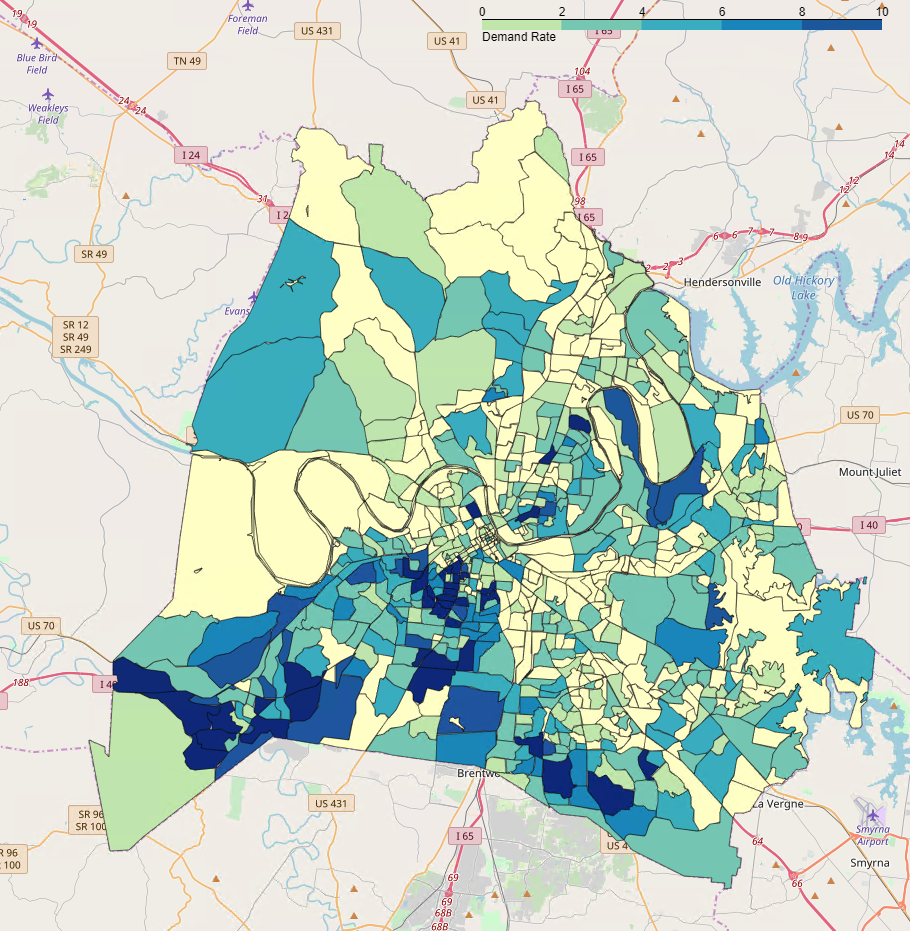
\includegraphics[width=.85\columnwidth]{taz_chloropeth.png}}
\caption{Vanderbilt University traffic demand distribution.}
\label{fig:demand_dist}
\end{center}
\vspace{-0.3in}
\end{figure}
\fi




%\Aron{This paragraph is just one sentence.}
In this section, we describe a simulated carpooling scenario. The problem of carpooling assignment was introduced earlier in Section~\ref{sec:carpoolingprob}.
%the implementation of the carpooling problem (Section~\ref{sec:carpoolingprob}).
Here, we model a carpool prosumer as an actor that specifies
\begin{enumerate*}
    \item whether it is providing or requesting a ride,
    \item the number of seats being offered/requested,
    \item a residence,
    \item a destination,
    \item a time interval during which the ride is available/required,
    \item and a radius specifying how far out of their way they are willing to travel.
\end{enumerate*}
%and is able to submit offers based on these factors. 
To setup the carpooling problem, we need to identify these parameters and encode them as offers. 

\begin{figure}[t]
\centering
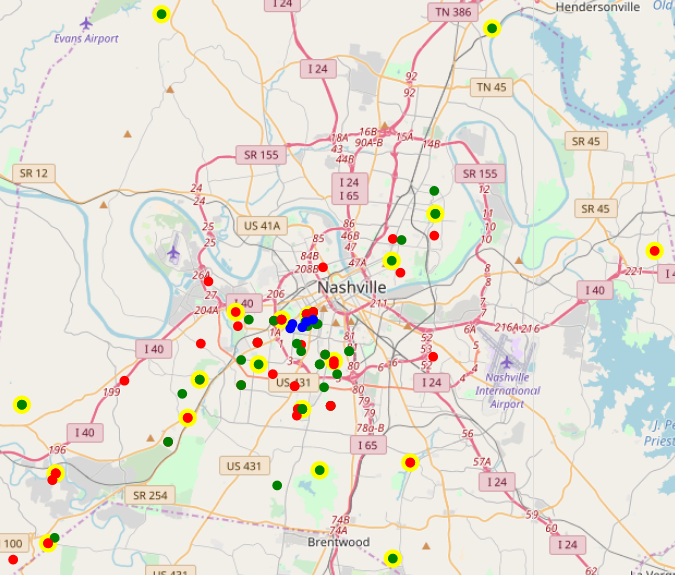
\includegraphics[width=0.7\columnwidth]{figs/clusters.png}
\caption{
%Distribution of riders, carpool locations, and destinations. 
Green and red dots mark the 75 residences (anonymized and resampled). Blue dots are destinations on campus. We used K-Means to identify 20 central locations (yellow dots) for pickup.
%from which providers and consumers travel. Blue dots are destinations on campus. We used K-Means to identify 20 central locations (yellow dots) for pickup. At this zoom level, some of the red and green points overlap and hide each other.
}
\label{fig:clusters}
\end{figure}

Residences were generated by sampling from real-trip distribution data of Vanderbilt 
\ifExtended
University, see Figure~\ref{fig:demand_dist}.
\else
University.
\fi
\ifExtended
This data provides Traffic Analysis Zone (TAZ)\footnote{TAZ is a special area delineated by state and/or local transportation officials for tabulating traffic-related data, especially journey-to-work and place-of-work statistics.} level data for trips taken from different parts of the city to the main university campus.
\fi
Destinations were chosen uniformly at random for each prosumer from the~5 garages around Vanderbilt University.
Other parameters were also chosen randomly:  number of seats from the range of 1 to 3,  prosumer type from producer or consumer,  time interval from 15-minute intervals between 7:00 and 9:30AM. The ``out of the way'' metric was chosen to be half of the distance between the residence and the destination. For a provider, the center of the pick-up circle is the midway point between the residence and the destination, and for a consumer,  the center is the residence.

Since each prosumer has a distinct residence, encoding it as a unique resource type would mean that every  prosumer would need to have the address of every other prosumer to determine if they are in their pick-up range. Instead, we specify \textit{pick-up points} which are public locations were carpoolers can meet. Each prosumer can determine which pick-up points are within their out-of-the-way radius and list those points in their offer. To encode these values, we assign an ID to each pickup point and destination. Finally, we encode each 15-minute interval using a timestamp. %s in the time range specified. 

An offer consists of a collection of alternative resource types, each with a quantity and value.
We encode a resource type, which is a combination of a time interval, a pick-up point, and  a destination, as a 64-bit unsigned integer. %The generic form of this resource type is ``timestampSrcIdDstId'', and specific instance is 152362170053 where the
For example, if timestamp is 1523621700,  pick-up location ID is 15, and destination ID is 3, then the resource type is 1523621700153. %An offer can be composed of multiple resource types and so we include one for combination of 15 minute interval and pick up point within range. An example of a full 
A complete offer may look as follows: 
%{64, True, 55, {1523623500173: 2, 1523621700153: 2, 152362440053: 2, 1523624400173: 2}, {1523623500173: 10, 1523621700153: 10, 152362440053: 10, 1523624400173: 10}.
%\footnotesize{
%\vspace{-0.1in}
\begin{align*}
      \{ \texttt{True}, ~ %& \\
     & \{1523623500173: 2, %\\ 
        1523623500153: 2, \\
     &  ~\,1523624400153: 2, %\\
        1523624400173: 2\}, \\
     & \{1523623500173: 10, %\\ 
        1523623500153: 10, \\
     & ~\,1523624400153: 10, %\\
        1523624400173: 10\} ~\} .
\end{align*}
%\vspace{-0.1in}
%\normal
%
In this offer, the prosumer is offering rides (\texttt{True} for providing), has two pick-up locations in range (17 and 15), drives to destination 3, is available in two time intervals, offers 2 seats, and asks for value 10 in exchange for a ride. %It has 4 resource types, they specify 2 times (1523623500, 1523624400) and two pickup points (17, 15).  

%\Aron{This sentence seems to have been mixed up, I'm not sure what it is supposed to be.}
%We have used Vanderbilt University employees' trip distribution data for modeling agents used in our simulation. and \textbf{Traffic analysis zone (TAZ)} dataset from US Census \cite{census2016nashville} to model demand distribution of Vanderbilt employees in each TAZ. TAZ is a special area delineated by state and/or local transportation officials for tabulating traffic-related data, especially journey-to-work and place-of-work statistics. Based on the demand distribution in each TAZ, we have sampled random points in each TAZ based on likelihood. So, if one TAZ has 100 people and another TAZ has 1000 people, then the likelihood of picking people from the 1000-people TAZ will be 10 times higher than from the 100-people TAZ. Figure~\ref{fig:demand_dist} shows the demand rate of Vanderbilt employees in each TAZ.
In our experiment, we selected 75 prosumers for the carpool service simulation. The red and green points in Figure~\ref{fig:clusters} are the locations of the consumers and producers randomly sampled from the anonymized distribution data of employees of Vanderbilt University. The yellow points were selected as pick up locations using K-Means clustering choosing 20 clusters. The blue points are 5 garages around Vanderbilt campus where employees typically park.  

Figure \ref{fig:offers} shows all the offers posted to the carpool platform. Each color is a unique offer. For example, the providing offer that is represented by red bars on the first six columns (7:00--8:15AM) having a height of 2, offers 2 seats with pick-up any time between 7:00AM and 8:15AM. The offers are stacked, showing how many seats are potentially available at that time. The chart combines all start and end locations; however, these could be separated. 

\begin{figure}[t]
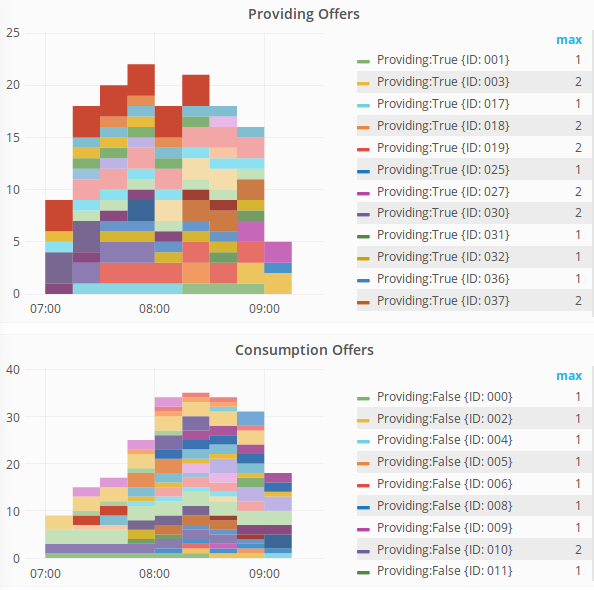
\includegraphics[width=\columnwidth]{figs/Offers.png}
\caption{Carpooling offers posted.}
\label{fig:offers}
\end{figure}

Figure \ref{fig:matches} shows the offers matched in each interval. For example, at 7:45AM, 2 providing offers--yellow (1 seat) and blue (1 seat)--and two consuming offers--yellow (1 seat) and orange (1 seat)--were matched. These are again grouped only by time in the figure, and not by start or end points. 
%This experiment was run on a \textcolor{red}{describe the machine}.  
%other runs solver: 18.3ms, 26.6ms
%other runs finzlize : 29s, 11.78s
The running time of the solver was $23$ ms, while the time between the request for finalization and emission of \texttt{AssignmentFinalized} events was $29$ s.
%

%between the receipt of the start finalize event and finalize completion event \Aron{I still don't understand, what is the ``start finalize event''? What is the ``finalize completion event''? When the contract emits AssignmentFinalized? When it is mined?} was $0.00039$ seconds. 

%Note that in this experiment, we are running our own private Ethereum blockchain network~\cite{EthereumBook}.

\begin{figure}[t]
\centering
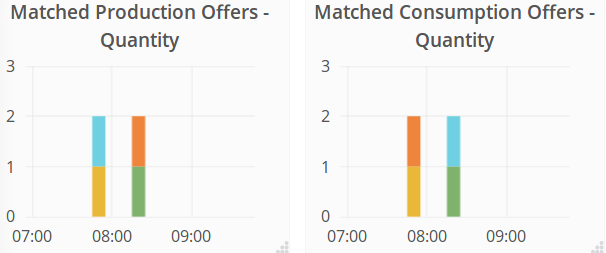
\includegraphics[width=0.9\columnwidth]{figs/matches.png}
\caption{Matched (i.e., assigned) offers in the solution.}
\label{fig:matches}
\end{figure}

% Table \ref{tab:timing} shows the measured time taken to solve the system of equations and the time between the receipt of the start finalize event and finalize completion event. 
% \begin{table}[t]
%     \centering
%     \caption{Performance Timings}
%     \label{tab:timing}
%     \renewcommand{\arraystretch}{1.2}
%     \begin{tabular}{|c|c|}
%         \hline
%         Solve Time & .0233s \\
%         \hline
%         Finalize Time & 0.00039s\\
%         \hline
%     \end{tabular}
% \end{table}

\begin{figure}[t]
    \centering
% \vspace{-0.1in}
%    \makebox[\linewidth]{
    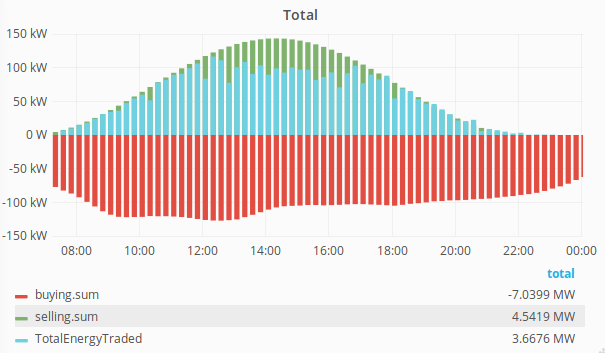
\includegraphics[width=0.95\linewidth]{totals.png}
%    }
    %\vspace{-0.2em}
    \caption{Total energy production capacity (green) and energy demand (red) for each interval, as well as the total energy traded in each interval (blue).}
    \label{fig:totals}
\end{figure}

\ifExtended
\begin{figure}[t]
\centering
    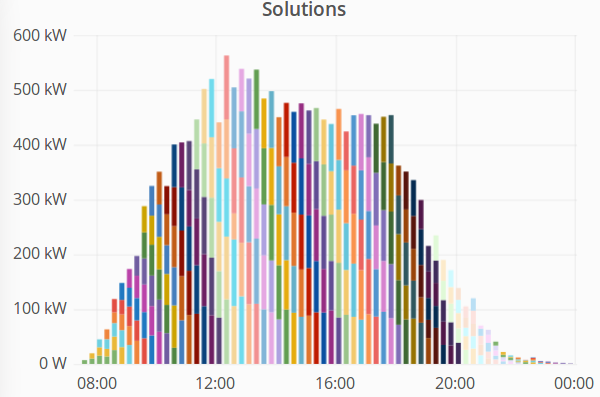
\includegraphics[width=0.95\linewidth]{figs/MultipleSolutions_white.png}
%    }
    %\vspace{-0.2em}
    \caption{\Platform recomputes the  solution for each future interval as more information becomes available. Each interval is finalized 2 cycles before it has to be actuated on the microgrid. The top stack for each interval is the ``finalized'' solution.}
    \label{fig:MultipleSolutions}
 
%     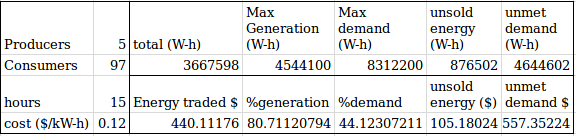
\includegraphics[width=1.0\linewidth]{totals_numbers.png}
% %    }
%     %\vspace{-0.2em}
%     \caption{Monetary impact of trades assuming a cost of \$0.12 per KWH }
%     \label{fig:monetary}
    %\vspace{-0.12in}
\end{figure}
 \fi 
 \ifExtended
 
\begin{figure}[t]
    \centering
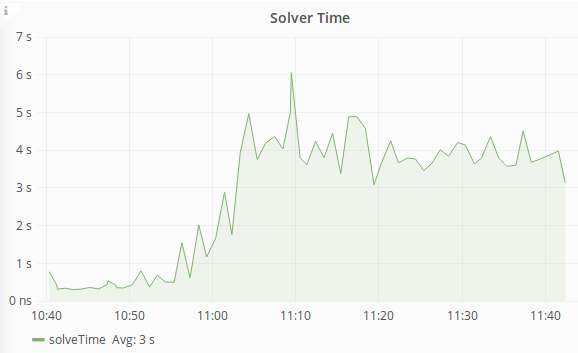
\includegraphics[width=\linewidth]{solveTime.png}
    \caption{ Running time of the solver for each cycle}
    \label{fig:solve-time}
% \end{subfigure}%
%  \begin{subfigure}{.5\columnwidth}
%   \centering
%   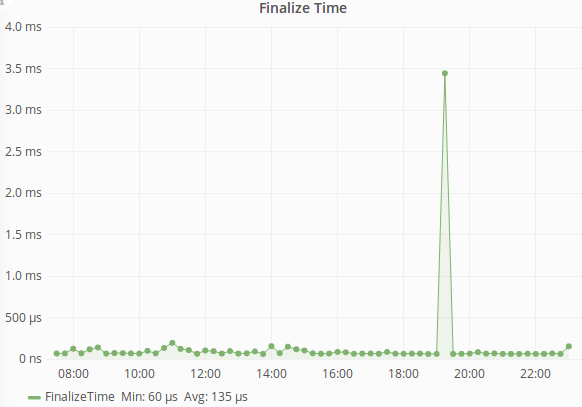
\includegraphics[width=\linewidth]{FinalizeTime.png}
% \caption{}
%   \label{fig:finalize-time}
% \end{subfigure}   
%\caption{ Running time of the solver for each cycle.}
%(b) Time for smart contract to finalize a trade}  
\end{figure}
\fi
\begin{figure} [h]
    \centering
% \vspace{-0.1in}
%    \makebox[\linewidth]{
    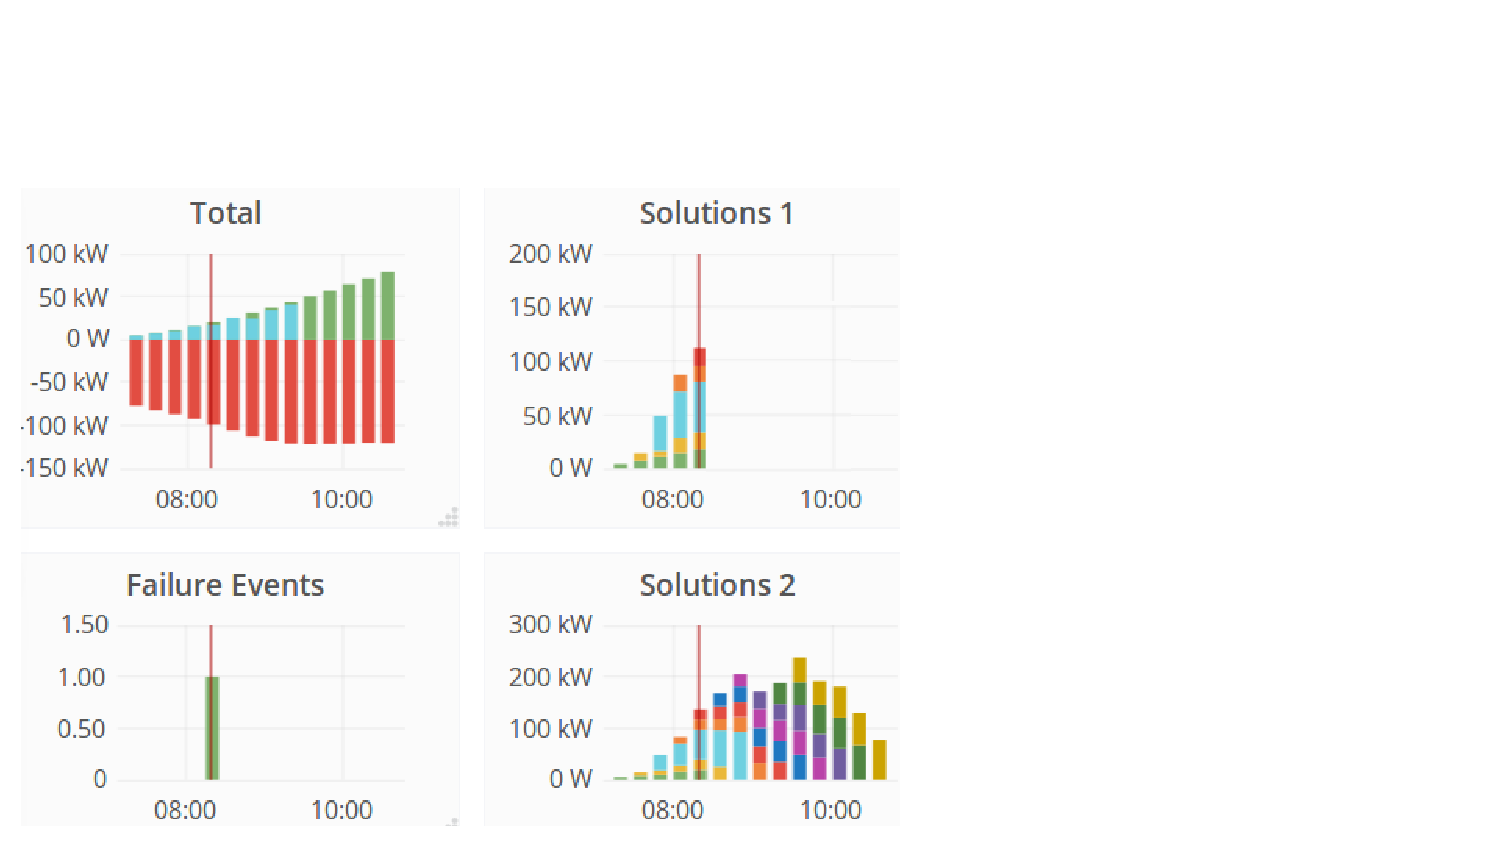
\includegraphics[width=0.9\linewidth]{failure.pdf}
%    }
    %\vspace{-0.2em}
    \caption{A failure scenario with failure at 8:15AM. The solver can submit new solutions as time progresses; the most recent solution is the color that is on the top of the stack for an interval.}
    \label{fig:failure}
    \vspace{-0.05in}
\end{figure}


% \begin{figure} [t]
%     \centering
% % \vspace{-0.1in}
% %    \makebox[\linewidth]{
%     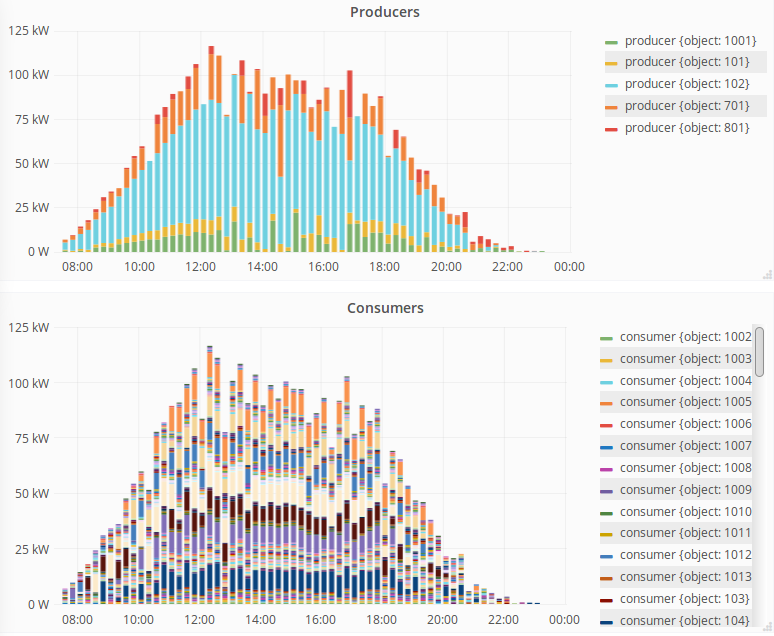
\includegraphics[width=1.0\linewidth]{trades.png}
% %    }
%     %\vspace{-0.2em}
%     \caption{Shows finalized solution for the amount of energy each prosumer is expected to produce(top) or consume(bottom) during each interval}
%     \label{fig:trades}
%     %\vspace{-0.12in}
% \end{figure}



\subsection{Energy Trading Problem}
 \label{sec:energy}

  To show the versatility of our transaction management platform, we now apply it to the problem of energy trading  within a microgrid, which we introduced in Section~\ref{sec:energyFuturesMarket}.
  %which we described in \cite{Laszka17}\Aron{We should mention what we did in~\cite{Laszka17} if we reference it.}.  
\ifExtended
  A key feature of this problem is peer-to-peer energy trading within microgrids to reduce the load on  distribution system operators (DSO) \cite{kok2016society,cox2013structured,melton2013gridwise}.  Such mechanisms can improve system reliability and efficiency by integrating inverter-based renewable resources into the grid and  supplying power to local loads when the main grid is interrupted.
  \fi
%  % !TeX root = ICCPS18.tex
  \definecolor{blueLine}{RGB}{57,106,177}
\definecolor{blueFill}{RGB}{114,147,203}
\definecolor{redLine}{RGB}{204,37,41}
\definecolor{greenline}{RGB}{0,250,0}
\definecolor{blackLine}{RGB}{0,0,0}
\definecolor{goldLine}{RGB}{160,82,45}
 
     \begin{figure}[t]
 \centering
\resizebox{0.45\textwidth}{!}{%
 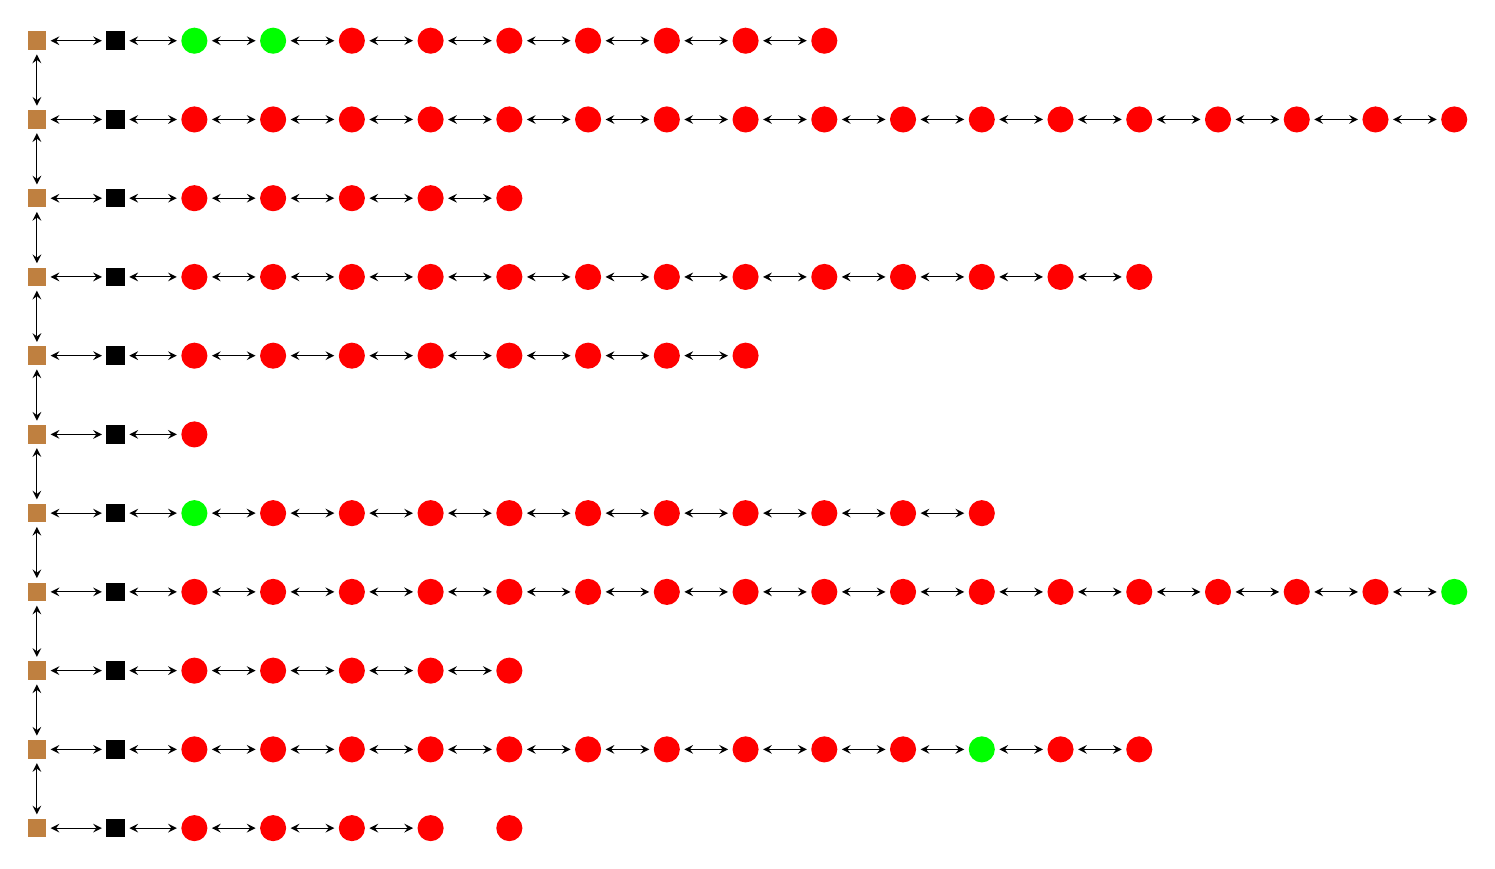
\begin{tikzpicture}[rotate=270,font=\tiny,
   oc/.style={fill=black,rectangle,minimum size=0.01cm,font=\tiny},
     feeder/.style={fill=brown,rectangle,minimum size=0.005cm,font=\tiny},
   Producer/.style={fill=green,circle,minimum size=0.01cm},
     Consumer/.style={fill=red,circle,minimum size=0.01cm},
   Connection/.style={<->, >=stealth, shorten <=0.05cm, shorten >=0.05cm}]
 \draw node[oc] (oc1) at (-5,0){};
 \draw node[oc] (oc2) at (-4,0){};
 \draw node[oc] (oc3) at (-3,0){};
 \draw node[oc] (oc4)  at (-2,0){};
 \draw node[oc](oc5)  at (-1,0){};
 \draw node[oc] (oc6)  at (0,0){};
 \draw node[oc] (oc7) at (1,0){};
 \draw node[oc] (oc8)  at (2,0){};
 \draw node[oc] (oc9) at (3,0){};
 \draw node[oc] (oc10) at (4,0){};
 \draw node[oc] (oc11) at (5,0){};

 \draw node[feeder] (feeder1) at (-5,-1){};
 \draw node[feeder] (feeder2) at (-4,-1){};
 \draw node[feeder] (feeder3) at (-3,-1){};
 \draw node[feeder] (feeder4)  at (-2,-1){};
 \draw node[feeder](feeder5)  at (-1,-1){};
 \draw node[feeder] (feeder6)  at (0,-1){};
 \draw node[feeder] (feeder7) at (1,-1){};
 \draw node[feeder] (feeder8)  at (2,-1){};
 \draw node[feeder] (feeder9) at (3,-1){};
 \draw node[feeder] (feeder10) at (4,-1){};
 \draw node[feeder] (feeder11) at (5,-1){};

 \draw [Connection] (feeder1) to (feeder2);
 \draw [Connection] (feeder2) to (feeder3);
 \draw [Connection] (feeder3) to (feeder4);
 \draw [Connection] (feeder4) to (feeder5);
 \draw [Connection] (feeder5) to (feeder6);
 \draw [Connection] (feeder6) to (feeder7);
 \draw [Connection] (feeder7) to (feeder8);
 \draw [Connection] (feeder8) to (feeder9);
 \draw [Connection] (feeder9) to (feeder10);
 \draw [Connection] (feeder10) to (feeder11);

\draw [Connection] (feeder1) to (oc1);
\draw [Connection] (feeder2) to (oc2);
\draw [Connection] (feeder3) to (oc3);
\draw [Connection] (feeder4) to (oc4);
\draw [Connection] (feeder5) to (oc5);
\draw [Connection] (feeder6) to (oc6);
\draw [Connection] (feeder7) to (oc7);
\draw [Connection] (feeder8) to (oc8);
\draw [Connection] (feeder9) to (oc9);
\draw [Connection] (feeder10) to (oc10);
\draw [Connection] (feeder11) to (oc11);


 \foreach \pos in {1,2} {
   \node [Producer] (p10\pos)at (-5,\pos) {};
 }

 \foreach \pos in {3,4,5,6,7,8,9} {
   \node [Consumer] (c10\pos)at (-5,\pos) {};
 }

 \foreach \pos in {1,2,3,4,5,6,7,8,9,10,11,12,13,14,15,16,17} {
   \node [Consumer] (c20\pos)at (-4,\pos) {};
 }

 \foreach \pos in {1,2,3,4,5} {
   \node [Consumer] (c30\pos)at (-3,\pos) {};
 }


 \foreach \pos in {1,2,3,4,5,6,7,8,9,10,11,12,13} {
   \node [Consumer] (c40\pos)at (-2,\pos) {};
 }


 \foreach \pos in {1,2,3,4,5,6,7,8} {
   \node [Consumer] (c50\pos)at (-1,\pos) {};
 }


 \foreach \pos in {1} {
   \node [Consumer] (c60\pos)at (0,\pos) {};
 }


 \foreach \pos in {1} {
   \node [Producer] (p70\pos)at (1,\pos) {};
 }


 \foreach \pos in {2,3,4,5,6,7,8,9,10,11} {
   \node [Consumer] (c70\pos)at (1,\pos) {};
 }


 \foreach \pos in {17} {
   \node [Producer] (p80\pos)at (2,\pos) {};
 }

 \foreach \pos in {1,2,3,4,5,6,7,8,9,10,11,12,13,14,15,16} {
   \node [Consumer] (c80\pos)at (2,\pos) {};
 }

 \foreach \pos in {1,2,3,4,5} {
   \node [Consumer] (c90\pos)at (3,\pos) {};
 }

 \foreach \pos in {11} {
   \node [Producer] (p100\pos)at (4,\pos) {};
 }

 \foreach \pos in {1,2,3,4,5,6,7,8,9,10,12,13} {
   \node [Consumer] (c100\pos)at (4,\pos) {};
 }

 \foreach \pos in {1,2,3,4,5} {
   \node [Consumer] (c110\pos)at (5,\pos) {};
 }


 \draw [Connection] (oc1) to (p101);
 \draw [Connection] (p101) to (p102);
 \draw [Connection] (p102) to (c103);
 \draw [Connection] (c103) to (c104);
 \draw [Connection] (c104) to (c105);
 \draw [Connection] (c105) to (c106);
 \draw [Connection] (c106) to (c107);
 \draw [Connection] (c107) to (c108);
 \draw [Connection] (c108) to (c109);
 
\draw [Connection] (oc2) to (c201);
\draw [Connection] (c201) to (c202);
\draw [Connection] (c202) to (c203);
\draw [Connection] (c203) to (c204);
\draw [Connection] (c204) to (c205);
\draw [Connection] (c205) to (c206);
\draw [Connection] (c206) to (c207);
\draw [Connection] (c207) to (c208);
\draw [Connection] (c208) to (c209);
\draw [Connection] (c209) to (c2010);
\draw [Connection] (c2010) to (c2011);
\draw [Connection] (c2011) to (c2012);
\draw [Connection] (c2012) to (c2013);
\draw [Connection] (c2013) to (c2014);
\draw [Connection] (c2014) to (c2015);
\draw [Connection] (c2015) to (c2016);
\draw [Connection] (c2016) to (c2017);

\draw [Connection] (oc3) to (c301);
\draw [Connection] (c301) to (c302);
\draw [Connection] (c302) to (c303);
\draw [Connection] (c303) to (c304);
\draw [Connection] (c304) to (c305);

\draw [Connection] (oc4) to (c401);
\draw [Connection] (c401) to (c402);
\draw [Connection] (c402) to (c403);
\draw [Connection] (c403) to (c404);
\draw [Connection] (c404) to (c405);
\draw [Connection] (c405) to (c406);
\draw [Connection] (c406) to (c407);
\draw [Connection] (c407) to (c408);
\draw [Connection] (c408) to (c409);
\draw [Connection] (c409) to (c4010);
\draw [Connection] (c4010) to (c4011);
\draw [Connection] (c4011) to (c4012);
\draw [Connection] (c4012) to (c4013);

\draw [Connection] (oc5) to (c501);
\draw [Connection] (c501) to (c502);
\draw [Connection] (c502) to (c503);
\draw [Connection] (c503) to (c504);
\draw [Connection] (c504) to (c505);
\draw [Connection] (c505) to (c506);
\draw [Connection] (c506) to (c507);
\draw [Connection] (c507) to (c508);

\draw [Connection] (oc6) to (c601);

\draw [Connection] (oc7) to (p701);
\draw [Connection] (p701) to (c702);
\draw [Connection] (c702) to (c703);
\draw [Connection] (c703) to (c704);
\draw [Connection] (c704) to (c705);
\draw [Connection] (c705) to (c706);
\draw [Connection] (c706) to (c707);
\draw [Connection] (c707) to (c708);
\draw [Connection] (c708) to (c709);
\draw [Connection] (c709) to (c7010);
\draw [Connection] (c7010) to (c7011);

\draw [Connection] (oc8) to (c801);
\draw [Connection] (c801) to (c802);
\draw [Connection] (c802) to (c803);
\draw [Connection] (c803) to (c804);
\draw [Connection] (c804) to (c805);
\draw [Connection] (c805) to (c806);
\draw [Connection] (c806) to (c807);
\draw [Connection] (c807) to (c808);
\draw [Connection] (c808) to (c809);
\draw [Connection] (c809) to (c8010);
\draw [Connection] (c8010) to (c8011);
\draw [Connection] (c8011) to (c8012);
\draw [Connection] (c8012) to (c8013);
\draw [Connection] (c8013) to (c8014);
\draw [Connection] (c8014) to (c8015);
\draw [Connection] (c8015) to (c8016);
\draw [Connection] (c8016) to (p8017);

\draw [Connection] (oc9) to (c901);
\draw [Connection] (c901) to (c902);
\draw [Connection] (c902) to (c903);
\draw [Connection] (c903) to (c904);
\draw [Connection] (c904) to (c905);

\draw [Connection] (oc10) to (c1001);
\draw [Connection] (c1001) to (c1002);
\draw [Connection] (c1002) to (c1003);
\draw [Connection] (c1003) to (c1004);
\draw [Connection] (c1004) to (c1005);
\draw [Connection] (c1005) to (c1006);
\draw [Connection] (c1006) to (c1007);
\draw [Connection] (c1007) to (c1008);
\draw [Connection] (c1008) to (c1009);
\draw [Connection] (c1009) to (c10010);
\draw [Connection] (c10010) to (p10011);
\draw [Connection] (p10011) to (c10012);
\draw [Connection] (c10012) to (c10013);


\draw [Connection] (oc11) to (c1101);
\draw [Connection] (c1101) to (c1102);
\draw [Connection] (c1102) to (c1103);
\draw [Connection] (c1103) to (c1104);

 \end{tikzpicture}
 }
 \caption{Feeder diagram. Brown nodes are feeder junctions, numbered 1 to 11 from top to bottom.  Black nodes are the overcurrent relays, which ensure that the total power flowing in and out of the feeder is below 20 kW. The green nodes are the junction points for the producers ($5$), and the red nodes are junction points for the consumers ($97$). There are $102$ prosumers in total.}
 \label{fig:feeder}
 \end{figure}


  In this example, a prosumer is modeled as an actor with an energy generation and consumption profile for the near future. In practice, the generation profile would be typically derived from predictions based on the weather, energy generation capabilities, and the amount of battery storage available. The consumption profile would be derived from flexible power loads, like  washers and electric vehicles.  

To represent future generation or consumption at a certain time, % loads as offers to the platform the 
resource types encode %composing an offer would simply be the
timestamps for 15-minute intervals, during which the power will be generated or consumed. 
As an example, consider a battery that has 500 Wh energy, which could be discharged any time between 9AM and 10AM.
%A simplified example (using clock time, rather than epoch time) could be a batter has stored 500W-h of energy and makes it available from 9:00-10:00AM. 
This can be represented by an offer having resource types 900, 915, 930, and 945, specifying a quantity of 500 Wh for each.

 
 For our simulation, the prosumer energy profiles are load traces recorded by Siemens during a day from a microgrid in Germany, containing $102$ homes %across $11$ feeders 
 ($5$ producers and $97$ consumers). Since the dataset does not include prices, we assume reservation prices to be uniform in our experiments, and focus on studying the amount of energy traded and the performance of the system. %Table \ref{tab:prosumers}
%Figure~\ref{fig:feeder} describes the feeder structure, the number of participants per feeder, and  the feeder safety limits.

%Each trace was divided into 15-minute time intervals that the prosumer can sumbit as an offer.

Figure~\ref{fig:totals} shows the total production (green) and consumption (red) across this microgrid, as well as the total energy traded per interval (blue) using our platform. The horizontal axis shows the starting time for each of the $96$ intervals.


\ifExtended
In this implementation, the prosumers do not submit all of the offers simultaneously, instead they post offers for the 5 intervals beyond the current interval being finalized. The justification for this is that a prosumer may not know their energy profile for the entire day and may only be able to make accurate estimates for a few future intervals at a time. Similarly a solver may be implemented to create matches for only the interval being finalized or may ``look-ahead'' at future offers and create match that may not be optimal for the current interval but allows better matches to be made in the future. This is a trade off between the complexity of the problem and how close the solution is to the global optimum.
%In this implementation, our solver finds a match for the current interval while looking ahead at the next 4 intervals.
%This can be seen in Figure  \ref{fig:MultipleSolutions},
%Since additional offers are being submitted during the simulation 
\Aron{This will be very unclear to the reviewers since the platform described in this paper does not do this.}
\Scott{Is that a better explanation?}
% Since the prosumers have a schedule for their energy consumption, they can post offers for several intervals in the future. By including offers for multiple intervals, the solver can find assignments for future intervals.
% As more information becomes available over time, the solver may find better solutions, as shown by Figure \ref{fig:MultipleSolutions}.
\fi

\ifExtended
For example, in the first interval, the green solution is submitted, which includes a matching for then current interval (at 7:30AM) as well as the next four intervals.
%, 7:45, 8:00, 8:15, and 8:30. 
Then, in the second interval, the yellow solution is added, which supersedes the green solution for intervals at 8:00AM, 8:15AM, and 8:30AM because more offers are now available and a better solution may be found. %, it also adds a solution for the 8:45 interval. 
% In this simulation, the solver solves for the current interval to be finalized as well as the next 4 intervals. The number of additional intervals can be varied to trade off between solve time, and overall solution optimality. 
\fi

%The solver time in this casestudy was 3s on average. Compared to carpool problem, this problem has more variables

\ifExtended
Figure \ref{fig:solve-time} shows the running time of the solver.
%with the 4 interval look-ahead. 
The time on the horizontal axis is the actual clock time, which shows that the simulation ran for about an hour. We also note that at about 20 minutes from the beginning (i.e., around interval 48), %which corresponds to noon in the simulated time series, 
solving time begins to increase. 
This increase is due to offers being made that span multiple intervals, i.e there are multiple resource types as in our 500Wh example.
\fi
%These kind of offers are possible because some of the selling offers can be valid for a range of future intervals instead of requiring immediate consumption (thanks to battery storage). 
%\Aron{Again, the reviewer will have no idea what we are talking about here.}
%\Scott{Is that more clear?}

In another simulation, we exercise the hybrid solver architecture by running multiple solvers, and after some time, cause one to fail. This result is shown in Figure~\ref{fig:failure}. The narrow vertical red line indicates when solver 1 fails at 8:15AM. Up until that point, solver 1 submitted the green, yellow, light blue, orange solutions, with the final solution being red.% Since the solver computes matching for the subsequent four intervals.
%solver 1 has a solution for them but they are not improved as new information is available. 
On the other hand we see that solver 2 continues to provide solutions for later intervals. 

% %To evaluate the performance of our solution, we take the following measurements:  running time of the solver to find a potential solution; time taken by the smart contract to finalize an interval\Aron{What is included in this? How is it measured? Very uncler!};  percentage of demand that is met with trades;  percentage of supply that is consumed through trades. 

% Results are shown in Figure \ref{fig:totals}.
% \Aron{?}

% \Aron{Font in figure is unreadable, it needs to be orders of magnitude bigger.}
% Figure \ref{fig:finalize-time} shows the time between the finalize event and the finalization of trades.

%The vertical narrow red line identifies the interval at 9:00am. In Solution 1 (), the purple bars were the last solution provided by Solver 1, while Solver 2 provides 4 more solutions during the next 4 intervals. 






%\Aron{We should move the detailed descriptions from the figure captions into the main text!}
 
\section{Related Research}
\label{sec:related}
%!TEX root = paper.tex
\section{Related Work}
\label{sec:related}

%In this section we describe the related research. It has been divided into two subsections to focus on blockchains, which we are using to implement the distributed ledger service described earlier, and other works on smart grid privacy concerns. 

%\subsection{Smart Grid and Meter Privacy}
% http://ieeexplore.ieee.org/abstract/document/5054916/
%McDaniel and McLaughlin discuss privacy challenges in smart grids~\cite{mcdaniel2009security}.
% https://arxiv.org/pdf/1108.2234.pdf
% https://pdfs.semanticscholar.org/cdf8/a5b6256823bca38a1d2347ab36f8e4a2ca94.pdf
% http://www.comm.toronto.edu/~akhisti/sm.pdf
% https://www.researchgate.net/profile/Georgios_Kalogridis/publication/224189766_Smart_Grid_Privacy_via_Anonymization_of_Smart_Metering_Data/links/541169510cf2b4da1bec4193.pdf
% https://arxiv.org/pdf/1305.0735.pdf
New privacy concerns arise with the continuing adoption of smart
grids. In addition to old and new security threats (such as energy
theft and smart-meter malware), McDaniel and McLaughlin discuss the
privacy concerns of energy usage profiling that smart grids could
potentially enable~\cite{mcdaniel2009security}. Several approaches
have been investigated as potential means to provide privacy
protections for smart grid users.

Some approaches look to the use of protocols and/or frameworks to help
protect privacy. Rajagopalan et al.\ use tools from information theory
to present a framework that abstracts both the privacy and the utility
requirements of smart-meter
data~\cite{rajagopalan2011smart,sankar2013smart}. Their framework
leads to a novel tractable privacy-utility tradeoff problem with
minimal assumptions. Efthymiou and Kalogridis describe a method for
securely anonymizing frequent electrical metering data sent by a smart
meter~\cite{efthymiou2010smart}. Their approach is based on the
observation that frequent metering data may be required by an energy
distribution network for operational reasons, but it may not
necessarily need to be attributable to a specific smart meter. The
authors describe a method that provides a third-party escrow mechanism
for authenticated anonymous meter readings, which are hard to
associate with a particular smart meter.

Other approaches, such as additional hardware components, are explored
for potential privacy gains. Varodayan and Khisti study using a
rechargeable battery for partially protecting the privacy of
information contained in a household's electrical load
profile~\cite{varodayan2011smart}. They show that stochastic battery
policies may leak 26\% less information than a best-effort policy,
which holds the output load constant whenever possible. Tan et
al.\ study privacy in a smart metering system from an information
theoretic perspective in the presence of energy harvesting and storage
units~\cite{tan2013increasing}. They show that energy harvesting
provides increased privacy by diversifying the energy source, while a
storage device can be used to increase both energy efficiency and
privacy.
% They show that there exists a trade-off between the information
% leakage rate and the wasted energy rate, and study the impact of the
% energy harvesting rate and the size of the storage device on this trade-off.

PETra extends this earlier work by (1) leveraging a decentralized IoT
system for transactive energy and (2) addressing the novel privacy
threat posed by trading. In particular, while earlier work protected
the prosumers' privacy from the DSO, PETra also protects it from other
prosumers, as well as outside attackers.

A key element of PETra is its ability to distribute information among
peers via blockchains.  As blockchain technology develops and matures,
new frameworks, services, and protocols are being developed to
leverage the distributed ledgers provided by blockchains. For example,
Hyperledger Fabric is a platform for distributed ledger solutions,
which was designed to support pluggable implementations of different
components~\cite{hyperledger2017fabric}.
%Bitcoin Lightning Network is
%decentralized system, in which transactions are sent over a network of
%micropayment channels, whose transfer of value occurs
%off-blockchain~\cite{poon2016bitcoin}. 
Since this paper focuses on the theoretical foundations of PETra, any
of these distributed ledgers provide the required capabilities.

%\Abhishek{Aron this section should end with a few sentence about how our approach fits in. Perhaps just a few sentences reworded from introduction will be sufficient}

\iffalse
\subsection{Blockchains as Distributed Ledgers}

As Blockchain technology continues to develop and mature, new
frameworks, services, and protocols are being developed to leverage
blockchain's distributed ledger. Microsoft offers Blockchain as a
Service (BaaS) on Azure. Additionally, Microsoft has Project Bletchley
as its architectural approach to building an Enterprise Consortium
Blockchain Ecosystem, introducing two new concepts: blockchain
middleware and a secure means for calling code or data outside a
SmartContract or blockchain called
cryptlets~\cite{gray2016introducing}. Hyperledger Fabric is a platform
for distributed ledger solutions, which was designed to support
pluggable implementations of different
components~\cite{hyperledger2017fabric}. Bitcoin Lightning Network is
decentralized system, in which transactions are sent over a network of
micropayment channels whose transfer of value occurs
off-blockchain~\cite{poon2016bitcoin}. Interledger is a protocol for
payments across payment systems, which enables anyone with accounts on
two ledgers to create a connection between
them~\cite{thomas_protocol}. Xu et al.\ discuss the use of two pools
of proxy agents, an agreement pool and a payment pool, to assist in
protection of privacy when using blockchain technologies for
transactions on tangible goods~\cite{Xu2017}.  \fi

%\url{https://geli.net/residential/}
%\url{https://www.greentechmedia.com/articles/read/geli-raises-7m-to-take-energy-storage-software-to-the-next-level}

%\url{http://ethembedded.com/}

\section{Conclusion}
\label{sec:conclusion}

% Section 7
% Conclusion:
% - discussion 
% - future work?

%\color{red}

Smart and connected community applications require decentralized and scalable platforms due to the large number of participants and the lack of mutual trust between them. In this paper,  we introduced a transactive platform for resource allocation, called \Platform. We first formulated a general problem that can be used to represent a variety of resource allocation problems in smart and connected communities. Then, we described an efficient and trustworthy platform based on a hybrid approach, which combines the efficiency of traditional computing environments with the trustworthiness of blockchain-based smart contracts. Finally, we demonstrated the applicability of our platform using two case studies based on real-world data.

% Challenges in smart and connected communities: lack of trust, large number of participants, distributed system \newline
% To overcome these challenges, in this paper,
% \begin{itemize}
%     \item we introduced a transactive platform for resource allocation
%     \item we formulated a general problem that can be used to represent resource allocation problems in various smart and connected communities
%     \item we described an efficient and trustworthy platform based on a hybrid approach that combines the efficiency of traditional computing environments with the trustworthiness of blockchain based smart contracts
%     \item we evaluated and demonstrated the applicability of our platform using two case studies based on real-world data
% \end{itemize}
% \color{black}

\vspace{0.5em}
\noindent\textbf{Acknowledgement:}
This work was funded in part by a grant from Siemens, CT and in part by a grant from NSF under award number CNS-1647015.


\let\oldbibliography\thebibliography
\renewcommand{\thebibliography}[1]{\oldbibliography{#1}
\setlength{\itemsep}{0pt}} %Reducing spacing in the bibliography.


\bibliographystyle{IEEEtran}
%\setlength{\bibsep}{0.0pt}
\small{
\bibliography{references} 
}

%\newpage
%\tableofcontents


\end{document}